\documentclass[10pt,openany]{article}
\usepackage{ctex} 
\usepackage{geometry,graphicx,xcolor,color}
\geometry{
	a4paper,
	top=25.4mm, bottom=25.4mm,
	left=20mm, right=20mm,
	headheight=2.17cm,
	headsep=4mm,
	footskip=12mm
}
\usepackage[all,pdf]{xy}
\usepackage{amssymb,amsmath,mathrsfs}             
\usepackage{mathpazo}
\usepackage[nofontspec]{newpxtext}
\usepackage{array}
\usepackage{amsmath}
\usepackage{amssymb}
\usepackage{enumerate}
\usepackage{amsthm}
\usepackage{bm}
\usepackage{mathtools}
\usepackage{mathrsfs}
\usepackage{tcolorbox}
\usepackage{indentfirst}
\usepackage{setspace}
\usepackage{subfigure} 
\usepackage{tkz-fct}
\usetikzlibrary{calc,intersections,through,backgrounds,3d}
\usetikzlibrary{shapes,arrows}
\tikzstyle{startstop} = [rectangle,rounded corners, minimum width=3cm,minimum height=1cm,draw=black,fill=red!30]
\tikzstyle{io} = [trapezium, trapezium left angle = 70,trapezium right angle=110,minimum width=3cm,minimum height=1cm,text centered,draw=black,fill=blue!30]
\tikzstyle{process} = [rectangle,minimum width=4cm,minimum height=1cm,text centered,text width =4cm,draw=black,fill=red!30]
\tikzstyle{decision} = [diamond,minimum width=3cm,minimum height=1cm,text centered,draw=black,fill=green!30]
\tikzstyle{arrow} = [thick,->,>=stealth]

\usepackage{tkz-euclide}
\usepackage{tikz-3dplot}
\usepackage{pgfplots}
\usepackage{booktabs}
\usepackage{float}
\usepackage[graphicx]{realboxes}
\usepackage{fancyhdr}
\setcounter{MaxMatrixCols}{20}
\usepackage{nicematrix}
\definecolor{winered}{rgb}{0.5,0,0}
\definecolor{structurecolor}{RGB}{122,122,142}
\definecolor{main}{HTML}{3D445F}
\definecolor{second}{HTML}{627581}
\definecolor{third}{HTML}{333333}
\definecolor{deepgreen}{HTML}{2F5E4E}  
\definecolor{purple}{HTML}{512E5F}   

\usepackage{hyperref}
\hypersetup{colorlinks = true, linktoc=all, linkcolor=blue, urlcolor=winered}


\usepackage{amsthm}
\usepackage{xcolor}
\usepackage{etoolbox}
\newtheoremstyle{defstyle}
{0.3cm}{0.3cm}{\fangsong}{-1cm}{\bfseries\color{main}}{}{0.5em}
{\indent 【\thmname{#1} \thmnumber{#2}】\ifthenelse{\equal{#3}{}}{}{~\thmnote{(#3)}}}

\newtheoremstyle{thmstyle}
{0.3cm}{0.3cm}{\kaishu}{-1cm}{\bfseries\color{second}}{}{0.5em}
{\indent 【\thmname{#1} \thmnumber{#2}】\ifthenelse{\equal{#3}{}}{}{~\thmnote{(#3)}}}

\newtheoremstyle{remstyle}
{0.3cm}{0.3cm}{\kaishu}{-1cm}{\bfseries\color{third}}{}{0.5em}
{\indent 【\thmname{#1} \thmnumber{#2}】\ifthenelse{\equal{#3}{}}{}{~\thmnote{(#3)}}}

\newtheoremstyle{exastyle}
{0.3cm}{0.3cm}{\kaishu}{-1cm}{\bfseries\color{deepgreen}}{}{0.5em}
{\indent 【\thmname{#1} \thmnumber{#2}】\ifthenelse{\equal{#3}{}}{}{~\thmnote{(#3)}}}

\newtheoremstyle{prostyle}
{0.3cm}{0.3cm}{\kaishu}{-1cm}{\bfseries\color{purple}}{}{0.5em}
{\indent 【\thmname{#1} \thmnumber{#2}】\ifthenelse{\equal{#3}{}}{}{~\thmnote{(#3)}}}

\theoremstyle{thmstyle} %theorem style
\newtheorem{theorem}{定理}[subsection]
\newtheorem{practice}{练习}[section]
\theoremstyle{defstyle} % definition style
\newtheorem{definition}[theorem]{定义}
\newtheorem{algorithm}[theorem]{算法}
\newtheorem{defprop}[theorem]{定义\(-\)命题}
\newtheorem{lemma}[theorem]{引理}
\newtheorem{corollary}[theorem]{推论}
\theoremstyle{prostyle} % proposition style
\newtheorem{proposition}[theorem]{命题}
\newtheorem{property}[theorem]{性质}
\theoremstyle{exastyle} 
\newtheorem{example}[theorem]{例}
\AtEndEnvironment{example}{\hfill \( \diamondsuit \)}
\theoremstyle{remstyle} 
\newtheorem{remark}[theorem]{注}

\renewenvironment{proof}[1][证明]{\par\underline{\textbf{#1.}} \;\fangsong}{\qed\par}
\newenvironment{solution}{\par\underline{\textbf{解.}} \;\fangsong}{\qed\par}
\newcommand{\intro}[1]{\rightline{\parbox[t]{5cm}{\footnotesize \fangsong\quad\quad #1 }}}

\AtEndEnvironment{proof}{\vspace{1.5ex}}
\AtEndEnvironment{solution}{\vspace{1.5ex}}

\usepackage{titlesec, titletoc}
\linespread{1.2} 				
\usepackage{fancyhdr}
\fancyhf{}
\renewcommand{\headrule}{\color{structurecolor}\hrule width\textwidth}
\pagestyle{fancy}
\renewcommand{\headrulewidth}{1pt}
\fancypagestyle{plain}{\renewcommand{\headrulewidth}{0pt}\fancyhf{}\renewcommand{\headrule}{}}

\fancyhead[c]{\color{structurecolor}\kaishu\rightmark}
\fancyfoot[c]{\color{structurecolor}\small\thepage}


\titleformat{\section}[frame]{\normalfont\color{structurecolor}}{\footnotesize \enspace \large \textcolor{structurecolor}{\S \,\thesection}\enspace}{6pt}{\Large\filcenter \bf \kaishu }


\titleformat{\subsection}[hang]{\bfseries}{\large\bfseries\color{structurecolor}\thesubsection\enspace}{1pt}{\color{structurecolor}\large\bfseries\filright}

\titleformat{\subsubsection}[hang]{\bfseries}{\large\bfseries\color{structurecolor}\thesubsubsection\enspace}{1pt}{\color{structurecolor}\large\bfseries\filright}

\usepackage{titling}
\renewcommand*{\maketitle}{
	\begin{titlepage}
		\newgeometry{margin = 0in}
		\parindent=0pt
		\includegraphics[width=\linewidth]{cover.png}
		\vfill
		\begin{center}
			\parbox{0.618\textwidth}{
				\hfill {\bfseries \Huge \thetitle} \\[0.6pt]  
				\rule{0.618\textwidth}{4pt} \\ 
			}
		\end{center}
		\vfill
		\begin{center}
			\parbox{0.618\textwidth}{
				\hfill\Large
				\kaishu 
				\begin{tabular}{r|}
					\textbf{2025 Summer} \\
					作者:\theauthor \\ 
					时间:\thedate \\
				\end{tabular}
			}
		\end{center}
		\vfill
		\begin{center}
			\parbox[t]{0.7\textwidth}{\centering \kaishu}
		\end{center}
		\vfill
	\end{titlepage}
	\restoregeometry
	\thispagestyle{empty}
}

\newcommand{\T}{^{\text{T}}}
\newcommand{\Her}{^{\text{H}}}
\newcommand{\F}{\mathbb{F}}
\newcommand{\gfn}{\text{GL}_n(\mathbb{F})}
\newcommand{\gfm}{\text{GL}_m(\mathbb{F})}
\newcommand{\C}{\mathbb{C}}
\newcommand{\R}{\mathbb{R}}
\newcommand{\Q}{\mathbb{Q}}
\newcommand{\n}{^{n \times n}}
\newcommand{\mn}{^{m \times n}}
\newcommand{\nm}{^{n \times m}}
\newcommand{\leinv}{_\text{L}^{-1}}
\newcommand{\riinv}{_\text{R}^{-1}}
\newcommand{\tz}{\mathrm{char} \;} 
\newcommand{\tr}{\mathrm{tr}}
\newcommand{\diag}{\mathrm{diag}}
\newcommand{\bmxi}{\bm{\xi}}
\newcommand{\bmeta}{\bm{\eta}}
\newcommand{\bme}{\bm{e}}
\newcommand{\oneb}{\underline{\hspace{1em}}\hspace{0.001em}}
\newcommand{\twob}{\oneb\oneb}
\newcommand{\fourb}{\twob\twob}
\newcommand{\tenb}{\twob\twob\twob\twob\twob}
\newcommand{\tideparallel}{%  
	\mathrel{%  
		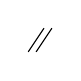
\begin{tikzpicture}[scale=0.2, baseline={([yshift=-0.5ex]current bounding box.center)}]  
			\draw[thin] (0,0) -- (1,1.5);  
			\draw[thin] (0.5,0) -- (1.5,1.5);  
		\end{tikzpicture}%  
	}%  
}  
\newcommand{\fourch}[4]
{\\[3pt]
	\begin{tabular}
		{*{4}{@{}p{4cm}}}
		A.~#1 & B.~#2 & C.~#3 & D.~#4
	\end{tabular}	
}
\newcommand{\fourchh}[4]
{\\[5pt]
	\begin{tabular}
		{*{4}{@{}p{20cm}}}
		A.~#1 \\[5pt] B.~#2 \\[5pt] C.~#3 \\[5pt] D.~#4
	\end{tabular}	
}
\newcommand{\fourchhh}[4]
{\\[3pt]
	\begin{tabular}
		{*{4}{@{}p{7.5cm}}}
		A.~#1 & B.~#2 \\[2pt] C.~#3 & D.~#4
	\end{tabular}	
}
\newcommand{\independent}{\perp\!\!\!\perp}
\everymath{\displaystyle}
\allowdisplaybreaks



\begin{document}

\pagestyle{fancy}
\lhead{Lecture 4}
\chead{illusion \& FzRainD}
\rhead{\today}

\setcounter{section}{3}

\section{Review of Chapter 1 Matrix}

回顾第一章的学习,我们以线性方程组的求解为主线,先提出了矩阵的乘法运算和分块矩阵运算,而后沿着公式解的线索引入可逆矩阵和行列式理论,最后探寻矩阵在初等变换下的不变量\(-\)秩,顺带用减号逆给出了更一般情形下的公式解.

\textbf{本节复习课的大部分习题选自《复旦大学高等代数习题集》和《高等代数学学习指导书(第四版)》谢启鸿 \ 姚慕生编著. 由于笔者懈怠,未标注具体页数,还请见谅. }

\subsection{行列式}

行列式虽然主要作为工具服务于线性方程组,但是它的求解技艺和题目是异常丰富的,在这里列举几类典型问题,适当练习即可,切勿沉迷其中.

在后续学习中,我们主要还是遇到低阶数字矩阵的行列式,一定牢记,用初等变换打洞求解是运算量最低的方法,一般我们不会使用组合定义,在运算过程中,适当观察使用性质会让计算更加简洁和轻松.

\subsubsection{按行/列展开,Laplace 定理和代数余子式问题}

对于有多个零的行列式我们一般选择直接展开计算,利用的就是行列式的归纳展开定义或者 Laplace 定理. 在代数余子式的计算上,回忆下面这个重要的结论.

\begin{proposition}
	设 \( A=(a_{ij}) \in \F\n \),设其古典伴随矩阵为 \( A^*=(A_{ji}) \in \F\n \),那么 \( AA^*=A^*A=(\det A)E_n \). 换言之,
	\[ \sum_{k=1}^{n} a_{ik}A_{ik}= \sum_{t=1}^{n} a_{tj}A_{tj}=\det A, \; \sum_{k=1}^{n} a_{ik}A_{jk}= \sum_{t=1}^{n} a_{ti}A_{tj}= 0 \ (i \neq j). \]
\end{proposition}

\begin{example} \label{4.1.2}
	设 
	\[ \det A = \begin{vmatrix}
		1 & 4 & 7 & \cdots & 3n-2 \\
		1 & 5 & 9 & \cdots & 4n-3 \\
		a_{31} & a_{32} & a_{33} & \cdots & a_{3n} \\
		\vdots & \vdots & \vdots & \ddots & \vdots \\
		a_{n1} & a_{n2} & a_{n3} & \cdots & a_{nn}
	\end{vmatrix}, \]
	
	证明:\( \det A= \sum_{i,j=1}^{n} A_{ij} \).
\end{example}

\begin{proof}
	将行列式按第一行展开
	\[ \sum_{j=1}^{n} a_{1j}A_{1j}= \sum_{j=1}^{n} (3j-2)A_{1j}= \det A, \; \sum_{j=1}^{n} a_{1j}A_{ij}=0 \ (2 \leq i \leq n), \]
	
	于是
	\begin{equation}
		\sum_{j=1}^{n}\sum_{i=1}^{n} (3j-2) A_{ij}=\det A. 
		\label{equa 4.1.1}
	\end{equation}
	
	同理,	将行列式按第二行展开
	\begin{equation}
	    \sum_{j=1}^{n}\sum_{i=1}^{n} (4j-3) A_{ij}=\det A.
	    \label{equa 4.1.2}
	\end{equation}
	
	\( 4 \times (\ref{equa 4.1.1})-3 \times (\ref{equa 4.1.2}) \) 可得
	\[ 4\det A-3\det A=\sum_{j=1}^{n}\sum_{i=1}^{n} [4(3j-2)-3(4j-3)] A_{ij} \leadsto \det A= \sum_{i,j=1}^{n} A_{ij}. \]
\end{proof}

矩阵的 Kronecker 积在后续处理类似 \( \varphi: X \mapsto AXB \) 或者 \( \varphi: X \mapsto AX-XB \) 此类的线性映射时会派上用场,从几何的角度来看,它描述了两个线性映射的张量积在基下的表示矩阵. 在此我们先接受其定义,并研究一些简单的性质.

\begin{example}
	设 \( A \in \F\n, \; B \in \F^{m \times m} \),定义矩阵 \( A,B \) 的 Kronecker 积为 \( A \otimes B \) 为 \( \F \) 上的 \( nm \times nm \) 矩阵
	\[ A \otimes B := \begin{bmatrix}
		a_{11}B & a_{12}B & \cdots & a_{1n}B \\
		a_{21}B & a_{22}B & \cdots & a_{2n}B \\
		\vdots & \vdots & \ddots & \vdots \\
		a_{n1}B & a_{n2}B & \cdots & a_{nn}B
	\end{bmatrix}, \]
	
	\begin{enumerate}[(1)]
		\item 用 Laplace 定理说明 \( \det (A \otimes E_m)= (\det A)^m, \; \det (E_n \otimes B)=(\det B)^n \);
		\item 验证 \( A \otimes B=(A \otimes E_m)(E_n \otimes B) \),进而有 \( \det (A \otimes B)= (\det A)^m (\det B)^n \).
	\end{enumerate}
	
\end{example}


\begin{proof}
	(1) 注意到 \( E_n \otimes B \) 就是分块对角矩阵 \( \diag\{B,B,\cdots,B\} \). 那么 \( \det (E_n \otimes B)=(\det B)^n \). 对 \( A \otimes E_m \),按第 \( 1, n+1,2n+1,\cdots,(m-1)n+1 \) 行展开,由 Laplace 定理
	\[ \det(A \otimes E_m)=(-1)^{2[1+\cdots+(m-1)n+1]} \det A \det(A \otimes E_{m-1})=\det A \det(A \otimes E_{m-1}). \]
	
	以此类推. (2) 任取 \( A \otimes B \) 的 \( (p,q) \) 元,作 \( \mathbb{Z} \) 上的带余除法 \( p=(i-1)m+s, \; q=(j-1)m+t, \; 0<s,t<m, \; i,j \in \mathbb{N} \). 只需要验证 \( (A \otimes B)_{p,q}=a_{ij}b_{st} \) 即可. 注意 \( A \otimes E_m \) 的第 \( p \) 行元素形如
	\[ \alpha\T= (A \otimes E_m)_{p,-}=\begin{bNiceMatrix}[last-row] 
		0 & \cdots & a_{i1} & \cdots & a_{i2} & \cdots & a_{ij} & \cdots & a_{in} & \cdots & 0 \\ 
		& & s & & m+s & & (j-1)m+s & & (n-1)m+s & & 
		\end{bNiceMatrix}, \]
	
	\( E_n \otimes B \) 的第 \( q \) 列元素形如
	\[ \beta=(E_n \otimes B)_{-,q}=\begin{bNiceMatrix}[last-col]
		0 & \\ \vdots & \\ 0 & (j-1)m \\ b_{1t} & (j-1)m+1 \\ b_{2t} & (j-1)m+2  \\ \vdots & \vdots \\ b_{st} & (j-1)m+s \\ \vdots & \vdots  \\ b_{mt} & jm  \\ 0  & \\ \vdots &  \\ 0 & 
	\end{bNiceMatrix}, \]
	
	于是 \( (A \otimes B)_{p,q}=\alpha\T\beta= a_{ij}b_{st} \). 那么 \( A \otimes B=(A \otimes E_m)(E_n \otimes B) \).
\end{proof}

\begin{practice}
	已知
	\[ \begin{vmatrix}
		1 & 2 & 3 & 4 & 5 \\
		2 & 2 & 2 & 1 & 1 \\
		3 & 1 & 2 & 4 & 5 \\
		1 & 1 & 1 & 2 & 2 \\
		4 & 3 & 1 & 5 & 0
	\end{vmatrix}=27. \]
	
	求 \( A_{21}+A_{22}+A_{23} \) 和 \( A_{24}+A_{25} \).
\end{practice}

\begin{solution}
	注意行列式第二行和第四行的特殊性,可以列方程组
	\[ \left\{ \begin{array}{l}
		2(A_{21}+A_{22}+A_{23})+1(A_{24}+A_{25})=27, \\
		1(A_{21}+A_{22}+A_{23})+2(A_{24}+A_{25})=0.
	\end{array}\right. \leadsto \left\{ \begin{array}{l}
	A_{21}+A_{22}+A_{23}=18, \\
	A_{24}+A_{25}=-9.
	\end{array}\right. \]
	
	这类似例 \ref{4.1.2}.
\end{solution}


\subsubsection{基本性质,加边法,求和法,拆分法}

在讲义 2 的小节 \S 2.2.4 一些计算实例 I, 这三类方法和基本性质的运用已经练习得比较多,我们只再举两个经典的习题.

\begin{example} \label{4.1.4}
	给定循环行列式
	\[ \det A = \begin{vmatrix}
		1 & 2 & 3 & \cdots & n \\
		n & 1 & 2 & \cdots & n-1 \\
		n-1 & n & 1 & \cdots & n-2 \\
		\vdots & \vdots & \vdots & \ddots & \vdots \\
		2 & 3 & 4 & \cdots & 1
	\end{vmatrix}, \]
	
	(1) 求 \( \det A \); (2) 求 \( \sum_{i,j=1}^{n} A_{ij} \).
\end{example}

\begin{solution}
	(1) 将第 \( n, n-1, \cdots, 2 \) 行都加到第一行,提取公因子 \( n(n+1)/2 \) 得到
	\[ \det A = \frac{n(n+1)}{2}\begin{vmatrix}
		1 & 1 & 1 & \cdots & 1 \\
		n & 1 & 2 & \cdots & n-1 \\
		n-1 & n & 1 & \cdots & n-2 \\
		\vdots & \vdots & \vdots & \ddots & \vdots \\
		2 & 3 & 4 & \cdots & 1
	\end{vmatrix}. \]
	
	接着用第 \( n \) 列减去 \( n-1 \) 列,第 \( n-1 \) 列减去第 \( n-2 \) 列,\( \cdots \),第 \( 2 \) 列减去第 \( 1 \) 列
	\[ \det A = \frac{n(n+1)}{2}\begin{vmatrix}
		1 & 0 & 0 & \cdots & 0 \\
		n & 1-n & 1 & \cdots & 1 \\
		n-1 & 1 & 1-n & \cdots & 1 \\
		\vdots & \vdots & \vdots & \ddots & \vdots \\
		2 & 1 & 1 & \cdots & 1-n
	\end{vmatrix}. \]
	
	这属于加边形式,真正要求的就是右下角的 \( n-1 \) 阶行列式,更换第一列方便求解
	\[ \det A = \frac{n(n+1)}{2}\begin{vmatrix}
		1 & 0 & 0 & \cdots & 0 \\
		1 & 1-n & 1 & \cdots & 1 \\
		1 & 1 & 1-n & \cdots & 1 \\
		\vdots & \vdots & \vdots & \ddots & \vdots \\
		1 & 1 & 1 & \cdots & 1-n
	\end{vmatrix}= \frac{n(n+1)}{2}\begin{vmatrix}
	1 & -1 & -1 & \cdots & -1 \\
	1 & -n & 0 & \cdots & 0 \\
	1 & 0 & -n & \cdots & 0 \\
	\vdots & \vdots & \vdots & \ddots & \vdots \\
	1 & 0 & 0 & \cdots & -n
	\end{vmatrix}. \]
	
	回到爪型行列式
	\[ \det A= \frac{n(n+1)}{2}\begin{vmatrix}
		1-\frac{n-1}{n} & -1 & -1 & \cdots & -1 \\[2ex]
		0 & -n & 0 & \cdots & 0 \\
		0 & 0 & -n & \cdots & 0 \\
		\vdots & \vdots & \vdots & \ddots & \vdots \\
		0 & 0 & 0 & \cdots & -n
	\end{vmatrix}= (-n)^{n-1} \cdot \frac{1}{n} \cdot \frac{n(n+1)}{2}= \frac{n+1}{2} (-n)^{n-1}. \]
	
	(2) 熟知
	\[ \sum_{i=1}^{n}\sum_{j=1}^{n} a_{kj}A_{ij}= \det A, \; \forall \; 1 \leq k \leq n. \]
	
	上式对 \( k \) 求和,我们已知
	\[ \sum_{k=1}^{n} a_{kj}= \frac{n(n+1)}{2} \leadsto n\det A= \frac{n(n+1)}{2} \sum_{i,j=1}^{n} A_{ij}. \]
	
	于是
	\[ \sum_{i,j=1}^{n} A_{ij}=(-n)^{n-1}. \]
\end{solution}


\begin{example} \label{4.1.5}
	设 \( f_1(x), f_2(x), \cdots, f_n(x) \in \F[x] \) 且 \( f_i(x) \) 的次数 \( \deg f_i(x) \) 都不超过 \( n-2 \; (1 \leq i \leq n)\),证明:对任意 \( n \) 个数 \( a_1,\cdots,a_n \in \F \) 都有
	\[ \begin{vmatrix}
		f_1(a_1) & f_2(a_1) & \cdots & f_n(a_1) \\
		f_1(a_2) & f_2(a_2) & \cdots & f_n(a_2) \\
		\vdots & \vdots & \ddots & \vdots \\
		f_1(a_n) & f_2(a_n) & \cdots & f_n(a_n)
	\end{vmatrix}=0. \]
\end{example}

\begin{proof}
	每一列的形式无非就是 \( 1,a_i,\cdots,a_i^{n-2} \) 附带某个 \( \F \) 系数的和,利用行列式的加法性质,最多可以把原行列式拆分为 \( (n-1)^n \) 个每一列都为单项式的行列式的和. 现在研究拆分后的行列式,如果想要非零,那么每一列都必须是 \( a_i \) 的不同次幂,否则两列成比例直接导出零. 然而所有可能出现的项中,一共只有 \( n-1 \) 种 \( a_i \) 的不同次幂,但是行列式有 \( n \) 列,故这 \( (n-1)^n \) 个行列式全部为零,原行列式值也即为零.
\end{proof}


\begin{practice}
	计算如下的 \( n \) 阶行列式,其中 \( n \geq 3 \).
	\[ \det A= \begin{vmatrix}
		1 & 2 &  \cdots & n-1 & n \\
		1 & 1 &  \cdots & 1 &  n-1 \\
		1 & 1 &  \cdots & n-1 & 1 \\
		\vdots & \vdots & \ddots  & \vdots & \vdots \\
		1 & n-1 & \cdots & 1 & 1
	\end{vmatrix}. \]
\end{practice}

\begin{solution}
	用第 \( n \) 列减去 \( n-1 \) 列,第 \( n-1 \) 列减去第 \( n-2 \) 列,\( \cdots \),第 \( 2 \) 列减去第 \( 1 \) 列
	\[ \det A= \begin{vmatrix}
		1 & 1 & 1 &  \cdots & 1 & 1 \\
		1 & 0 & 0 &  \cdots & 0 &  n-2 \\
		1 & 0 & 0 & \cdots & n-2 & 2-n \\
		\vdots & \vdots & \vdots & \ddots  & \vdots & \vdots \\
		1 & 0 & n-2 & \cdots & 0 & 0 \\
		1 & n-2 & 2-n & \cdots & 0 & 0
	\end{vmatrix}. \]
	
	接下来用第 \( 2 \) 行加到第 \( 3 \) 行,第 \( 3 \) 行加到第 \( 4 \) 行,\( \cdots \),第 \( n-1 \) 行加到第 \( n \) 行
	\[ \det A= \begin{vmatrix}
		1 & 1 & 1 &  \cdots & 1 & 1 \\
		1 & 0 & 0 &  \cdots & 0 &  n-2 \\
		2 & 0 & 0 & \cdots & n-2 & 0 \\
		\vdots & \vdots & \vdots & \ddots  & \vdots & \vdots \\
		2 & 0 & n-2 & \cdots & 0 & 0 \\
		2 & n-2 & 0 & \cdots & 0 & 0
	\end{vmatrix}. \]
	
	用类似爪型行列式的手段将第一列从第二行起打为零
	\[ \det A= \begin{vmatrix}
		1-\frac{2(n-2)}{n-2}-\frac{1}{n-2} & 1 & 1 &  \cdots & 1 & 1 \\[2ex]
		0 & 0 & 0 &  \cdots & 0 &  n-2 \\
		0 & 0 & 0 & \cdots & n-2 & 0 \\
		\vdots & \vdots & \vdots & \ddots  & \vdots & \vdots \\
		0 & 0 & n-2 & \cdots & 0 & 0 \\
		0 & n-2 & 0 & \cdots & 0 & 0
	\end{vmatrix}=\begin{vmatrix}
	\frac{1-n}{n-2} & 1 & 1 &  \cdots & 1 & 1 \\[2ex]
	0 & 0 & 0 &  \cdots & 0 &  n-2 \\
	0 & 0 & 0 & \cdots & n-2 & 0 \\
	\vdots & \vdots & \vdots & \ddots  & \vdots & \vdots \\
	0 & 0 & n-2 & \cdots & 0 & 0 \\
	0 & n-2 & 0 & \cdots & 0 & 0
	\end{vmatrix}. \]
	
	用组合定义展开即
	\[ \det A= (-1)^{\sigma(1,n,n-1\cdots,2)}(1-n)(n-2)^{n-2}=(-1)^{(n-2)(n-1)/2}(1-n)(n-2)^{n-2}. \]
	
	本练习类似例 \ref{4.1.4}.
\end{solution}


\subsubsection{递推公式和数学归纳法}

递推公式的典例就是如下的三对角行列式. 在讲义 2 的小节 \S 2.2.4 一些计算实例 I 我们也有使用过递推公式法,不过一般太难观察出来,实际应用需要灵感.

\begin{example}
	设
	\[
	D_n =
	\begin{bmatrix}
		a+b & ab   &        &        &        \\
		1   & a+b  & ab     &        &        \\
		& 1    & a+b    & ab     &        \\
		&      & \ddots & \ddots & \ddots \\
		&      &        & 1      & a+b
	\end{bmatrix}, \quad n \geq 3.
	\]
	
	求 \( \det D_n \).
\end{example}

\begin{solution}
	按第一列展开,
	\begin{align*}
		D_n&= (a+b)\begin{vmatrix}
			a+b & ab   &        &        &        \\
			1   & a+b  & ab     &        &        \\
			& 1    & a+b    & ab     &        \\
			&      & \ddots & \ddots & \ddots \\
			&      &        & 1      & a+b
		\end{vmatrix}_{n-1}+(-1)^{1+2} \begin{vmatrix}
			ab   &        &        &        \\
			1    & a+b    & ab     &        \\
			& \ddots & \ddots & \ddots \\
			&        & 1      & a+b
		\end{vmatrix}_{n-1} \\
		&= (a+b)D_{n-1}-(ab)\begin{vmatrix}
			a+b & ab   &        &        &        \\
			1   & a+b  & ab     &        &        \\
			& 1    & a+b    & ab     &        \\
			&      & \ddots & \ddots & \ddots \\
			&      &        & 1      & a+b
		\end{vmatrix}_{n-2}=(a+b)D_{n-1}-(ab)D_{n-2}.
	\end{align*}

   这是一个二阶常系数齐次线性递推. 考虑特征方程 \( x^2-(a+b)x+ab=(x-a)(x-b)=0 \). 当 \( ab=0 \) 时,\( D_n \) 显然. 下面只考虑 \( ab \neq 0 \). 当 \( a \neq b \) 时,可以设 \( D_n=\lambda_1 a^n+ \lambda_2 b^n \; (\lambda_i \in \F) \). 求两个初值 \( D_1=a+b, \; D_2=a^2+b^2+ab \). 于是
   \[ \left\{ \begin{array}{l}
   	\lambda_1 a+ \lambda_2 b = a+b, \\
   	\lambda_1 a^2+ \lambda_2 b^2= a^2+b^2+ab.
   \end{array}\right. \leadsto  \left\{ \begin{array}{l}
   \lambda_1=1+b(a-b)^{-1}=a(a-b)^{-1}, \\
   \lambda_2=1+a(b-a)^{-1}=(-b)(a-b)^{-1}.
   \end{array}\right. \]
   
   那么 
   \[ D_n=\frac{a^{n+1}-b^{n+1}}{a-b}. \]
   
   当 \( a = b \neq 0 \) 时,可以设 \( D_n=(\lambda_1n+\lambda_2)a^n \; (\lambda_i \in \F)  \). 于是
   \[ \left\{ \begin{array}{l}
   	(\lambda_1+\lambda_2)a = 2a, \\
   	(2\lambda_1+\lambda_2)a^2= 3a^2.
   \end{array}\right. \leadsto  \left\{ \begin{array}{l}
   	\lambda_1=1, \\
   	\lambda_2=1.
   \end{array}\right. \]
   
   那么 \( D_n=(n+1)a^n \).
\end{solution}


下面的例题事实上是在求解 Frobenius 块的特征多项式,读者应该对这个结论留有印象,我们在相似标准形章节会直接应用这个结论.

\begin{example}
	设
	\[
	A_n =
	\begin{bmatrix}
		\lambda &        &        &        & a_n \\
		-1      & \lambda &       &        & a_{n-1} \\
		& -1     & \lambda &       & a_{n-2} \\
		&        & \ddots & \ddots & \vdots \\
		&        &        & -1     & \lambda + a_1
	\end{bmatrix}.
	\]
	
	求 \( \det A_n \).
\end{example}

\begin{solution}
	按第一行展开,
	\begin{align*}
		A_n&= \lambda \begin{vmatrix}
			\lambda &       &        & a_{n-1} \\
			-1     & \lambda &       & a_{n-2} \\
			& \ddots & \ddots & \vdots \\
			&        & -1     & \lambda + a_1
		\end{vmatrix}_{n-1}+ (-1)^{n+1} a_n \begin{vmatrix}
			-1      & \lambda &       &        \\
			& -1     & \lambda &        \\
			&        & \ddots & \vdots  \\
			&        &        & -1     
		\end{vmatrix}_{n-1} \\
		&= \lambda A_{n-1}+ (-1)^{n+1+n-1} a_n= \lambda A_{n-1}+ a_n
	\end{align*}
   
   这是一个一阶变系数齐次线性递推. 注意 \( a_n \) 依赖于下标 \( n \). 我们尝试用数学归纳法给出通项公式. 初步计算 \( A_1=\lambda+a_1, \; A_2= \lambda(\lambda+a_1)-(-1)a_2=\lambda^2+a_1\lambda+a_2 \). 归纳假设 \( A_k= \lambda^k+a_1\lambda^{k-1}+\cdots+a_{k-1}\lambda+a_k \). 利用递推公式,
   \[ A_{k+1}=  \lambda A_k+ a_{k+1}= \lambda^{k+1}+a_1\lambda^{k}+\cdots+a_{k}\lambda+a_{k+1}. \]
   
   假设成立. 那么 \( A_n= \lambda^n+a_1\lambda^{n-1}+\cdots+a_{n-1}\lambda+a_n  \). 我们将这个结论换一种形式来写. 设多项式 \( f(\lambda)=\lambda^n+a_1\lambda^{n-1}+\cdots+a_{n-1}\lambda+a_n  \in \F[\lambda] \) 的 Frobenius 块为
   \[ \bm{F}(f(\lambda))= \begin{bmatrix}
   	0 &        &        &        & -a_n \\
   	1   & 0 &       &        & -a_{n-1} \\
   	& 1     & 0 &       & -a_{n-2} \\
   	&        & \ddots & \ddots & \vdots \\
   	&        &        & 1     & -a_1
   \end{bmatrix}, \]
   
   那么 \( \det(\lambda E_n-\bm{F}(f(\lambda)))=f(\lambda) \).
\end{solution}

对于某些不确定性过多,无从下手的问题,数学归纳法可能派上用场.

\begin{example}
	证明:对于任意的方阵 \( H \in \F\n \),总存在任一使其对角元取 \( \pm 1 \) 的对角矩阵 \( J \in \F\n \),使得 \(\det(H + J) \neq 0 \).
\end{example}

\begin{proof}
	对 \( H \) 的阶数 \( n \) 用归纳法. 当 \( n=1 \) 时,不妨 \( H=(h) \). 注意到 \( h+1 \) 和 \( h-1 \) 不同时为 0. 假设 \( n-1 \) 时结论成立,阶数为 \( n \) 的情形,对 \( H \) 分块,其中 \( H_1 \) 为 \( n-1 \) 阶方阵,\( \alpha,\beta \in \mathbb{F}^{n-1} \).
	\[ H=\begin{bmatrix}
		H_1 & \alpha \\ \beta^T & h_{nn}
	\end{bmatrix}. \] 
	
	由归纳假设,存在 \( J_1 \) 为主对角元全为 \( \pm 1 \) 的 \( n-1 \) 阶对角矩阵,使得 \( \det(H_1+J_1) \neq 0 \). 待定 \( \ell \in \{1,-1\} \),令 \( J=\diag \{ J_1, \ell\} \). 由降阶公式知 \( \det(H+J)=\det(H_1+J_1) \cdot (h_{nn}+\ell-\beta^T(H_1+J_1)^{-1}\alpha) \). 注意到 \( h_{nn}-\beta^T(H_1+J_1)^{-1}\alpha \) 为一个确定的数,那么同 \( n=1 \) 的情形证毕.
\end{proof}

\begin{example} \label{4.1.9}
	设 \( A \in \R\n \; (n \geq 3) \). 证明:
	\begin{enumerate}[(1)]
		\item 若 \( A \) 中每个元素的绝对值为 \( 1 \),则 \( |\det A| \leq (2n!)/3 \);
		\item 若 \( A \) 中每个元素的绝对值为 \( 2 \),则 \( |\det A| \leq (2^{n+1}n!)/3 \).
	\end{enumerate}
	
\end{example}

\begin{proof}
	(1) 先讨论 \( n=3 \) 的情形,由于左乘初等矩阵 \( E(i(-1)) \) 不改变 \( \det A \) 的绝对值,那么不妨设 \( A \) 的第 1 列全为 1. 再通过右乘初等矩阵 \( E(j(-1)) \) 将 \( A \) 的 \( (1,2) \) 元素和 \( (1,3) \) 元素设置为 \( -1 \). 接下来将第 1 列加到第 \( 2,3 \) 列,得到
	\[ |\det A|= \text{abs} \left( \begin{vmatrix}
		1 & 0 & 0 \\
		1 & a & b \\
		1 & c & d
	\end{vmatrix} \right), \; a,b,c,d \in \{0,2\}. \]
	
	这说明 \( ad=4 \) 或者 0,进而
	\[ |\det A| =|ad-bc| \leq 4=(2 \times 3!)/3. \]
	
	假设结论对任意 \( 3 \leq m<n \) 阶行列式成立,现在讨论 \( n \) 阶行列式的情形,对 \( \det A \) 按第一行展开,那么
	\[ |\det A|= \left| \sum_{k=1}^{n} a_{1k}A_{1k} \right| \leq \sum_{k=1}^{n} |M_{1k}| \leq n \times \frac{2(n-1)!}{3}= \frac{2n!}{3}. \]
	
	(2) 对 \( \det A \) 的每一行提取公因子 \( 2 \) 后划归到 (1) 的情形.
\end{proof}


\begin{example}
	设 \( b_1,\cdots,b_{n^2} \in \F \) 为 \( n^2 \; (n \geq 2) \) 个不同的数,证明:存在 \( b_1,\cdots,b_{n^2} \) 的某个全排列,记为 \( a_{11},\cdots,a_{nn} \),使得 \( \det(a_{ij})_{n \times n} \neq 0 \).
\end{example}

\begin{proof}
	当 \( n=2 \) 时,由于 \( b_1 \) 关于加法的逆元唯一,那么 \( b_2,b_3,b_4 \) 中至多有一个加上 \( b_1 \) 等于 0. 取 \( a_{11}=b_1 \),那么存在 \( a_{12} \in \{b_2,b_3,b_4\} \) 使得 \( a_{11}+a_{12} \neq 0 \). 于是
	\[ \begin{vmatrix}
		a_{11} & a_{12} \\
		a_{12} & a_{11}
	\end{vmatrix}= (a_{11}-a_{12})(a_{11}+a_{12}) \neq 0. \]
	
	那么 \( (a_{11},a_{12}), \; (a_{12},a_{11}) \) 构成 \( \F^2 \) 的一组基. 余下的两个数任意指定为 \( a_{21}, \; a_{22} \),至少有 \( (a_{21},a_{22}) \neq \bm{0} \). 断言 \( (a_{11},a_{12}), \; (a_{12},a_{11}) \) 之一与 \( (a_{21},a_{22}) \) 线性无关,否则若均线性相关,就存在 \( 0 \neq \lambda_1, \lambda_2 \in \F \) 使得 
	\[ (a_{21},a_{22})=\lambda_1 (a_{11},a_{12})= \lambda_2 (a_{12},a_{11}). \]
	
	也就说明
	\[ \left\{ \begin{array}{l}
		a_{11} \lambda_1+ a_{12} (-\lambda_2)=0, \\
		a_{12} \lambda_1+ a_{11} (-\lambda_2)=0
	\end{array}\right. \leadsto \begin{bmatrix}
	a_{11} & a_{12} \\
	a_{12} & a_{11}
	\end{bmatrix}\begin{bmatrix}
	\lambda_1 \\
	-\lambda_2
	\end{bmatrix}=O. \]
	
	注意到 \( (\lambda_1,-\lambda_2) \neq \bm{0} \),但上述方程不可能有非零解,矛盾. 那么选取 \( (a_{11},a_{12}), \; (a_{12},a_{11}) \) 中与 \( (a_{21},a_{22}) \) 线性无关的向量与之拼成一个行列式,这个行列式必定非零. 
	
	当 \( n \geq 3 \),归纳假设结论对 \( n-1 \) 阶行列式成立,对 \( n \) 阶情形,如果 \( n^2 \) 个数的所有全排列组成的行列式值都为零,下面推出矛盾.
	
	选定 \( a_{11}=b_1 \),由于 \( b_2+\cdots+b_{n-1}+b_n \) 和 \( b_2+\cdots+b_{n-1}+b_{n+1} \) 必然不同,可以选取其中之一与 \( b_1 \) 的和非零,不妨设 \( b_1+(b_2+\cdots+b_{n-1}+b_n) \neq 0 \). 选定 \( a_{1j}=b_j \; (2 \leq j \leq n) \). 现在余下的 \( n^2-n>(n-1)^2 \) 个不同的数中,由归纳假设可以选取其中 \( (n-1)^2 \) 个不同的数按一定排列组成一个非零行列式,设定为 \( a_{11} \) 的代数余子式,余下的 \( n-1 \) 个数任意排列在 \( n \) 阶行列式第一列的剩余位置. 这样构造出一个 \( n \) 阶行列式 \( \det A \). 
	
	这时,\( \det A=a_{11}A_{11}+\cdots+a_{1n}A_{1n}=0 \). 固定第 \( 2 \sim n \) 行不动,对调第 \( 1 \) 行中 \( a_{11} \) 和 \( a_{1j} \ (2 \leq j \leq n) \) 的位置,由反证假设,
	\[ a_{1j}A_{11}+\cdots+a_{11}A_{1j}+\cdots+a_{1n}A_{1n}=0. \]
	
	也就得到 \( a_{1j}A_{11}+a_{11}A_{1j}=a_{11}A_{11}+a_{1j}A_{1j} \leadsto (a_{1j}-a_{11})(A_{11}-A_{1j})=0 \),而 \( a_{1j}-a_{11} \neq 0 \),只能 \( A_{11}-A_{1j}=0 \). 这说明一开始
	\[ \det A=(a_{11}+\cdots+a_{1n})A_{11}=0, \]
	
	但 \( a_{11}+\cdots+a_{1n}, \; A_{11} \) 均非零,推翻假设. 也就是结论对 \( n \) 阶情形也成立.
	
	
\end{proof}

\subsubsection{最重要的模板法:Vandermonde 行列式}

Vandermonde 行列式常常以各种变形的形式出现,要灵活运用行列式的各种性质和方法来解决.

\begin{example}
	计算下列 \( n+1 \) 阶行列式的值:
	\[ \det A= 	\begin{vmatrix}
		0 & 1 & 1 & \cdots & 1 \\
		1 & a_1 & a_2 & \cdots & a_n \\
		-2 & a_1^{2} & a_2^{2} & \cdots & a_n^{2} \\
		\vdots & \vdots & \vdots & \ddots & \vdots \\
		(-1)^{n-1} n & a_1^{n} & a_2^{n} & \cdots & a_n^{n}
	\end{vmatrix}.\]
\end{example}

\begin{solution}
	设 \( A=(a_{ij}) \),其中每个 \( a_{ij} \) 都是关于 \( x \) 的可微函数. 由行列式的组合定义以及导数的乘法法则,容易得到下面的行列式求导公式
	\[ (\det A)'= \sum_{i=1}^{n} \begin{vmatrix}
		a_{11} & a_{12} & a_{13} & \cdots & a_{1n} \\
		\vdots & \vdots & \vdots & \ddots & \vdots \\
		a_{i1}' & a_{i2}' & a_{i3}' & \cdots & a_{in}' \\
		\vdots & \vdots & \vdots & \ddots & \vdots \\
		a_{n1} & a_{n2} & a_{n3} & \cdots & a_{nn} 
	\end{vmatrix} = \sum_{j=1}^{n} \begin{vmatrix}
		a_{11} & \cdots & a_{1j}' & \cdots & a_{1n} \\
		a_{21} & \cdots & a_{2j}' & \cdots & a_{2n} \\
		a_{31} & \cdots & a_{3j}' & \cdots & a_{3n} \\
		\vdots & \ddots & \vdots & \ddots & \vdots \\
		a_{n1} & \cdots & a_{nj}' & \cdots & a_{nn} 
	\end{vmatrix}. \]
	
	回到原题,设
	\[ f(x)= \begin{vmatrix}
		1 & 1 & 1 & \cdots & 1 \\
		x & a_1 & a_2 & \cdots & a_n \\
		x^2 & a_1^{2} & a_2^{2} & \cdots & a_n^{2} \\
		\vdots & \vdots & \vdots & \ddots & \vdots \\
		x^n & a_1^{n} & a_2^{n} & \cdots & a_n^{n}
	\end{vmatrix}=\prod_{1 \leq i<j \leq n}^{} (a_j-a_i) \cdot \prod_{k=1}^{n} (a_k-x). \]
	
	那么
	\[ f'(x)= \begin{vmatrix}
		0 & 1 & 1 & \cdots & 1 \\
		1 & a_1 & a_2 & \cdots & a_n \\
		2x & a_1^{2} & a_2^{2} & \cdots & a_n^{2} \\
		\vdots & \vdots & \vdots & \ddots & \vdots \\
		nx^{n-1} & a_1^{n} & a_2^{n} & \cdots & a_n^{n}
	\end{vmatrix} = -\prod_{1 \leq i<j \leq n}^{} (a_j-a_i) \cdot \sum_{k=1}^{n}  \prod_{t \neq k}^{} (a_t-x). \]
	
	所求 
	\[ \det A= f'(-1)= -\prod_{1 \leq i<j \leq n}^{} (a_j-a_i) \cdot \sum_{k=1}^{n}  \prod_{t \neq k}^{} (a_t+1). \]
\end{solution}


\begin{example} \label{4.1.12}
	计算下列 \( n \) 阶行列式的值:
	\[ \det A= \begin{vmatrix}
		1 & x_1 & \cdots & x_1^{n-2} & x_1^{n} \\
		1 & x_2 & \cdots & x_2^{n-2} & x_2^{n} \\
		\vdots & \vdots & \ddots & \vdots & \vdots \\
		1 & x_n & \cdots & x_n^{n-2} & x_n^{n}
	\end{vmatrix}. \]
\end{example}

\begin{solution}
	考虑引入不定元 \( t \) 并升阶行列式
	\[ \det A':=\begin{vmatrix}
		1 & x_1 & \cdots & x_1^{n-2} & x_1^{n-1} & x_1^{n} \\
		1 & x_2 & \cdots & x_2^{n-2} & x_2^{n-1} & x_2^{n} \\
		\vdots & \vdots & \ddots & \vdots & \vdots & \vdots \\
		1 & x_n & \cdots & x_n^{n-2} & x_n^{n-1} & x_n^{n} \\
		1 & t & \cdots & t^{n-2} & t^{n-1} & t^n
	\end{vmatrix}= \prod_{1 \leq i<j \leq n}^{} (x_j-x_i) \cdot \prod_{k=1}^{n} (t-x_k)=:f(t). \]
	
	考察 \( t^{n-1} \) 的系数,将 \( \det A' \) 按第 \( n+1 \) 行展开,其值应为 \( (-1)^{(n+1)+n} \det A= -\det A \). 另一方面,在 \( f(t) \) 中 \( t^{n-1} \) 的系数为
	\[ -\prod_{1 \leq i<j \leq n}^{} (x_j-x_i) \sum_{k=1}^{n} x_k= -\det A. \]
	
	从上式中解出
	\[ \det A= \prod_{1 \leq i<j \leq n}^{} (x_j-x_i) \sum_{k=1}^{n} x_k. \]
\end{solution}


\begin{example}
	计算下列 \( n \) 阶行列式的值:
	\[ \det A= \begin{vmatrix}
		1 & x_1 & \cdots & x_1^{n-2} & (x_2+x_3+\cdots+x_n)^{n} \\
		1 & x_2 & \cdots & x_2^{n-2} & (x_1+x_3+\cdots+x_n)^{n} \\
		\vdots & \vdots & \ddots & \vdots & \vdots \\
		1 & x_n & \cdots & x_n^{n-2} & (x_1+x_2+\cdots+x_{n-1})^{n}
	\end{vmatrix}. \]
\end{example}

\begin{solution}
	将 \( (i,n) \) 元写作
	\[ \left( \sum_{j \neq i}^{} x_j \right)^n= \left( \sum_{j=1}^{n} x_j-x_i \right)^n= \sum_{k=0}^{n} C_n^k (-x_i)^k \left( \sum_{j=1}^{n} x_j \right)^{n-k}. \]
	
	于是可以用原行列式的 \( 1 \sim (n-1) \) 列消去其中的绝大部分,只剩下
	\[ \sum_{{\color{red}k= n-1}}^{n} C_n^k (-x_i)^k \left( \sum_{j=1}^{n} x_j \right)^{n-k}=(-1)^{n-1} nx_i^{n-1} \left( \sum_{j=1}^{n} x_j \right)+ (-1)^n x_i^n. \]
	
	代入 \( \det A \) 并用行列式的加法性质拆分,并利用例 \ref{4.1.12} 得到
	\begin{align*}
		\det A &= (-1)^{n-1} n \prod_{1 \leq i \leq j \leq n}^{} (x_j-x_i) \sum_{k=1}^{n} x_k+ (-1)^n \prod_{1 \leq i<j \leq n}^{} (x_j-x_i) \sum_{k=1}^{n} x_k, \\
		&= (-1)^{n-1} (n-1) \prod_{1 \leq i \leq j \leq n}^{} (x_j-x_i) \sum_{k=1}^{n} x_k.
	\end{align*}
\end{solution}


\begin{practice}
	计算下列 \( n \) 阶行列式的值:
	\[ \det A= \begin{vmatrix}
		1 & x_1(x_1-a) & x_1^{2}(x_1-a) & \cdots & x_1^{n-1}(x_1-a) \\
		1 & x_2(x_2-a) & x_2^{2}(x_2-a) & \cdots & x_2^{n-1}(x_2-a) \\
		\vdots & \vdots & \vdots & \ddots & \vdots \\
		1 & x_n(x_n-a) & x_n^{2}(x_n-a) & \cdots & x_n^{n-1}(x_n-a)
	\end{vmatrix}. \]
\end{practice}


\begin{solution}
	(\textbf{法一})\ 这非常类似例 \ref{4.1.5},注意到要想行列式拆分出的子行列式非零,每一列对应的 \( x_i \) 的次幂必须互不相同,也就是必须为 \( 1,x_i,\cdots,x_i^n \) 中 \( n \) 个互不相同的幂次,且从左到右的幂次应该是递增的. 也即
	\[ \det A=  \sum_{i=1}^{n-1} \begin{vmatrix}
		1 & (-a)x_1 & \cdots & (-a)x_1^{i-1} & x_1^{i+1} & \cdots & x_1^{n} \\
		1 & (-a)x_2 & \cdots & (-a)x_2^{i-1} & x_2^{i+1} & \cdots & x_2^{n} \\
		\vdots & \vdots & \ddots & \vdots & \vdots & \ddots & \vdots \\
		1 & (-a)x_n & \cdots & (-a)x_n^{i-1} & x_n^{i+1} & \cdots & x_n^{n}
	\end{vmatrix}+ (-a)^{n-1} \begin{vmatrix}
	1 & x_1 & \cdots & x_1^{n-2} & x_1^{n-1} \\
	1 & x_2 & \cdots & x_2^{n-2} & x_2^{n-1} \\
	\vdots & \vdots & \ddots & \vdots & \vdots \\
	1 & x_n & \cdots & x_n^{n-2} & x_n^{n-1}
	\end{vmatrix}. \]
	
	为了处理上式的第一项,简单记为对 \( (-a)^{i-1}\det A_i \) 求和. 回到例 \ref{4.1.12},考察 \( t^i \) 的系数,在第 \( n+1 \) 行的展开式中,其系数为 \( (-1)^{n+1+i+1} \det A_i=(-1)^{n+i} \det A_i \),在 \( f(t) \) 中 \( t^i \) 的系数为
	\[ (-1)^{n-i} \prod_{1 \leq s<t \leq n}^{} (x_t-x_s) \sum_{1 \leq l_1<\cdots<l_{n-i} \leq n}^{} x_{l_1}x_{l_2}\cdots x_{l_{n-i}}= (-1)^{n+i} \det A_i. \]
	
	于是
	\[ \det A_i= \prod_{1 \leq s<t \leq n}^{} (x_t-x_s) \sum_{1 \leq l_1<\cdots<l_{n-i} \leq n}^{} x_{l_1}x_{l_2}\cdots x_{l_{n-i}}. \]
	
	那么
	\[ \det A= \prod_{1 \leq s<t \leq n}^{} (x_t-x_s) \left\{ \sum_{i=1}^{n-1} (-a)^{i-1}  \sum_{1 \leq l_1<\cdots<l_{n-i} \leq n}^{} x_{l_1}x_{l_2}\cdots x_{l_{n-i}}+ (-a)^{n-1} \right\}. \]
	
	(\textbf{法二})\ 考虑引入未定元 \( y \),升阶为如下的 \( n+1 \) 阶行列式
	\[ \det A':= \begin{vmatrix}
		1 & x_1-a & x_1(x_1-a) & x_1^{2}(x_1-a) & \cdots & x_1^{n-1}(x_1-a) \\
		1 & x_2-a & x_2(x_2-a) & x_2^{2}(x_2-a) & \cdots & x_2^{n-1}(x_2-a) \\
		\vdots & \vdots & \vdots & \vdots & \ddots & \vdots \\
		1 & x_n-a & x_n(x_n-a) & x_n^{2}(x_n-a) & \cdots & x_n^{n-1}(x_n-a) \\
		1 & y-a & y(y-a) & y^2(y-a) & \cdots & y^{n-1}(y-a)
	\end{vmatrix}. \]
	
	上述行列式显然只能拆分出一项
	\[ \det A'= \begin{vmatrix}
		1 & x_1 & \cdots & x_1^{n-1} & x_1^{n} \\
		1 & x_2 & \cdots & x_2^{n-1} & x_2^{n} \\
		\vdots & \vdots & \ddots & \vdots & \vdots \\
		1 & x_n & \cdots & x_n^{n-1} & x_n^{n} \\
		1 & y & \cdots & y^{n-1} & y^{n}
	\end{vmatrix}= \prod_{1 \leq s<t \leq n}^{} (x_t-x_s) \prod_{k=1}^{n} (y-x_k)=:g(y) \]
	
	当 \( a=0 \) 时,对比左右两端 \( y \) 的系数
	\[ (-1)^{n+1+2} \det A= (-1)^{n-1} \prod_{1 \leq s<t \leq n}^{} (x_t-x_s) \sum_{k=1}^{n} \prod_{j \neq k}^{} x_j. \]
	
	于是
	\[ \det A=\prod_{1 \leq s<t \leq n}^{} (x_t-x_s) \sum_{k=1}^{n} \prod_{j \neq k}^{} x_j. \] 
	
	当 \( a \neq 0 \) 时,我们知道 \( g(y) \) 的常数项由下面两部分组成
	\begin{align*}
	 & \qquad (-1)^n \prod_{1 \leq s<t \leq n}^{} (x_t-x_s) \prod_{k=1}^{n} x_k \\
	 &=	(-1)^{n+1+2}(-a) \det A+ (-1)^{n+1+1}\begin{vmatrix}
			 x_1-a & x_1(x_1-a) & \cdots & x_1^{n-1}(x_1-a) \\
			x_2-a & x_2(x_2-a)  & \cdots & x_2^{n-1}(x_2-a) \\
			\vdots & \vdots  & \ddots & \vdots \\
			 x_n-a & x_n(x_n-a) & \cdots & x_n^{n-1}(x_n-a) \\
		\end{vmatrix}, \\
		&= (-1)^{n} a\det A+ (-1)^n \prod_{k=1}^{n} (x_k-a) \prod_{1 \leq s<t \leq n}^{} (x_t-x_s).
	\end{align*}
	
	得到
	\[ \det A= a^{-1} \prod_{1 \leq s<t \leq n}^{} (x_t-x_s) \left\{ \prod_{k=1}^{n} x_k -\prod_{k=1}^{n} (x_k-a)  \right\}. \]
	
	为了验证法一和法二结果的等价性,\( a=0 \) 是显然的. 对 \( a \neq 0 \),作等价代数变形
	\begin{align*}
		a^{-1} \left\{ \prod_{k=1}^{n} x_k -\prod_{k=1}^{n} (x_k-a)  \right\} &= -a^{-1} \sum_{i=1}^{n} (-a)^i \sum_{1 \leq l_1<\cdots<l_{n-i} \leq n}^{} x_{l_1}\cdots x_{l_{n-i}}, \\
		&= (-a)^{n-1}-a^{-1} \sum_{i=1}^{n-1} (-a)^i \sum_{1 \leq l_1<\cdots<l_{n-i} \leq n}^{} x_{l_1}\cdots x_{l_{n-i}}, \\
		&= (-a)^{n-1}+ \sum_{i=1}^{n-1} (-a)^{i-1} \sum_{1 \leq l_1<\cdots<l_{n-i} \leq n}^{} x_{l_1}\cdots x_{l_{n-i}}.
	\end{align*}
\end{solution}


\begin{example} \label{4.1.14}
	设 \( \lambda_1,\lambda_2,\cdots,\lambda_n \in \C \) 满足
	\[ \left\{ \begin{array}{l}
		\lambda_1+\lambda_2+\cdots+\lambda_n = r,\\
		\lambda_1^{2}+\lambda_2^{2}+\cdots+\lambda_n^{2} = r,\\
		\qquad \vdots\\
		\lambda_1^{n}+\lambda_2^{n}+\cdots+\lambda_n^{n} = r,\\
		\lambda_1^{n+1}+\lambda_2^{n+1}+\cdots+\lambda_n^{n+1} = r,
	\end{array}\right.\]
	
	其中 \( r \in [0,n] \) 为整数. 证明:\( \lambda_1,\lambda_2,\cdots,\lambda_n \) 中有 \( r \) 个 \( 1 \),\( n-r \) 个 \( 0 \).
\end{example}

\begin{proof}
   令 \( \lambda_{n+1}=1 \),那么原方程组等价于
   \[ \left\{ \begin{array}{l}
   	\lambda_1+\lambda_2+\cdots+\lambda_n-r\lambda_{n+1} = 0,\\
   	\lambda_1^{2}+\lambda_2^{2}+\cdots+\lambda_n^{2}-r\lambda_{n+1}^2 = 0,\\
   	\qquad \vdots\\
   	\lambda_1^{n}+\lambda_2^{n}+\cdots+\lambda_n^{n}-r\lambda_{n+1}^{n} = 0,\\
   	\lambda_1^{n+1}+\lambda_2^{n+1}+\cdots+\lambda_n^{n+1}-r\lambda_{n+1}^{n+1} = 0,
   \end{array}\right.\]
   
   反证. 若 \( \lambda_1,\lambda_2,\cdots,\lambda_n \) 中 1 的个数 \( N(1) \neq r \),将所有等于 \( 1 \) 的 \( \lambda_j \) 对应项 \( \lambda_j^i \) 与 \( -r\lambda_{n+1}^{i} \) 合并,合并后的系数为 \( N(1)-r \neq 0 \). 再将剩余的 \( \lambda_j \) 也按照取值相同的进行合并,若取值为 \( 0 \) 直接略去. 设整理后得到的方程为
    \[ (\text{I}) \left\{ \begin{array}{l}
    	N(\lambda_{j_1}) \lambda_{j_1}+\cdots+N(\lambda_{j_l})\lambda_{j_l}+(N(1)-r)\lambda_{n+1} = 0,\\
    	N(\lambda_{j_1}) \lambda_{j_1}^{2}+\cdots+N(\lambda_{j_l})\lambda_{j_l}^{2}+(N(1)-r)\lambda_{n+1}^2 = 0,\\
    	\qquad \vdots\\
    	N(\lambda_{j_1}) \lambda_{j_1}^{n}+\cdots+N(\lambda_{j_l})\lambda_{j_l}^{n}+(N(1)-r)\lambda_{n+1}^{n} = 0,\\
    	N(\lambda_{j_1}) \lambda_{j_1}^{n+1}+\cdots+N(\lambda_{j_l})\lambda_{j_l}^{n+1}+(N(1)-r)\lambda_{n+1}^{n+1} = 0,
    \end{array}\right.\]
    
    其中 \( N(\lambda_{j_k}) \geq 1 \),且 \( \lambda_{j_k} \neq 0,1 \) 两两不同. 取上述方程的前 \( 1 \sim (l+1) \) 个组成一个子方程组 (II),那么原方程组的解必定适合 (II)
    
    \[ (\text{II}) \left\{ \begin{array}{l}
    	N(\lambda_{j_1}) \lambda_{j_1}+\cdots+N(\lambda_{j_l})\lambda_{j_l}+(N(1)-r)\lambda_{n+1} = 0,\\
    	N(\lambda_{j_1}) \lambda_{j_1}^{2}+\cdots+N(\lambda_{j_l})\lambda_{j_l}^{2}+(N(1)-r)\lambda_{n+1}^2 = 0,\\
    	\qquad \vdots\\
    	N(\lambda_{j_1}) \lambda_{j_1}^{l}+\cdots+N(\lambda_{j_l})\lambda_{j_l}^{l}+(N(1)-r)\lambda_{n+1}^{l} = 0,\\
    	N(\lambda_{j_1}) \lambda_{j_1}^{l+1}+\cdots+N(\lambda_{j_l})\lambda_{j_l}^{l+1}+(N(1)-r)\lambda_{n+1}^{l+1} = 0,
    \end{array}\right.\]
    
    注意 (II) 系数矩阵的行列式为
    \[\left( \lambda_{n+1} \prod_{k=1}^{l} \lambda_{j_k}  \right) \prod_{1 \leq s < t \leq l}^{} (\lambda_{j_t}-\lambda_{j_s}) \cdot \prod_{k=1}^{l} (\lambda_{n+1}-\lambda_{j_k}) \neq 0. \]
    
    然而 \( (N(\lambda_{j_1}),\cdots,N(\lambda_{j_l}),N(1)-r)\T \) 给出了 (II) 的一个非零解,导出矛盾,说明 \( \lambda_1,\lambda_2,\cdots,\lambda_n \) 中 1 的个数 \( N(1)=r \). 再设 \( \lambda_1,\lambda_2,\cdots,\lambda_n \) 中 0 的个数 \( 0 \leq N(0)< n-r \). 用相同的方法得到方程组 (I)
    
     \[ (\text{I}) \left\{ \begin{array}{l}
    	N(\lambda_{j_1}) \lambda_{j_1}+\cdots+N(\lambda_{j_l})\lambda_{j_l}= 0,\\
    	N(\lambda_{j_1}) \lambda_{j_1}^{2}+\cdots+N(\lambda_{j_l})\lambda_{j_l}^{2}= 0,\\
    	\qquad \vdots\\
    	N(\lambda_{j_1}) \lambda_{j_1}^{n}+\cdots+N(\lambda_{j_l})\lambda_{j_l}^{n}= 0,\\
    	N(\lambda_{j_1}) \lambda_{j_1}^{n+1}+\cdots+N(\lambda_{j_l})\lambda_{j_l}^{n+1}= 0,
    \end{array}\right.\]
    
    其中 \( l \geq 1 \),因为 \( 0 \leq N(0)<n-r \). 同上选取前 \( l \) 个方程组成的子方程组,其存在非零解,但系数矩阵的行列式非零,矛盾.
\end{proof}

例 \ref{4.1.14} 可以用多项式章节的 Newton 公式得到一个简洁的证明. 不过在这里,我们只使用了 Vandermonde 行列式和 Cramer 法则. 这个例题最重要的应用是给出了判断幂零矩阵的一个充要条件,\( A \in \F\n \) 幂零当且仅当 \( \tr(A^i)=0 \ (1 \leq i \leq n+1) \),但具体的证明需要留到特征值章节.

\subsubsection{乘法法则,降阶公式和 Cauchy\(-\)Binet 公式}

降阶公式的习题已经在讲义 3 的小节 \S 3.2.3 中列举得非常丰富了,本小节主要需要应用聚焦乘法法则的问题. 这两种方法都需要你尝试将原本的矩阵进行拆分,需要一定的尝试. Cauchy\(-\)Binet 公式可以看成乘法法则的一般化.

\begin{example}
	设
	\[
	A =
	\begin{bmatrix}
		1 + x_1 y_1 & 1 + x_1 y_2 & \cdots & 1 + x_1 y_n \\
		1 + x_2 y_1 & 1 + x_2 y_2 & \cdots & 1 + x_2 y_n \\
		\vdots & \vdots & \ddots & \vdots \\
		1 + x_n y_1 & 1 + x_n y_2 & \cdots & 1 + x_n y_n
	\end{bmatrix}, \; n \geq 3.
	\]
	
	证明:\( \det A=0 \).
\end{example}

\begin{proof}
	(\textbf{法一}) \ 记
	\[ B=\begin{bmatrix}
		1 & x_1 \\
		1 & x_2 \\
		\vdots & \vdots \\
		1 & x_n 
	\end{bmatrix}, \; C=\begin{bmatrix}
	1 & 1 & \cdots & 1 \\
	y_1 & y_2 & \cdots & y_n
	\end{bmatrix}. \]
	
	于是 \( A=BC \). 由于 \( r(B) \leq 2 \),那么 \( r(A) \leq r(B) \leq 2<n \),只能 \( \det A=0 \). 这里也可以直接由 Cauchy\(-\)Binet 公式得到.
	
	\vspace{1ex}
	
	(\textbf{法二}) \ 记
	\[ B=\begin{bmatrix}
		1 & x_1 & 0 & \cdots & 0 \\
		1 & x_2 & 0 & \cdots & 0 \\
		1 & x_3 & 0 & \cdots & 0\\
		\vdots & \vdots & \vdots & \ddots & \vdots \\
		1 & x_n & 0 & \cdots & 0
	\end{bmatrix}, \; C=\begin{bmatrix}
		1 & 1 & 1 & \cdots & 1 \\
		y_1 & y_2 & y_3 & \cdots & y_n \\
		0 & 0 & 0 & \cdots & 0 \\
		\vdots & \vdots & \vdots  & \cdots & \vdots \\
		0 & 0 & 0 & \cdots & 0
	\end{bmatrix}. \]
	
	于是 \( A=BC \). 而 \( B,C \) 都是方阵,且 \( \det B=\det C=0 \). 直接由 Cauchy\(-\)Binet 公式得到.
\end{proof}


\begin{example}
	设 \( s_k = x_1^k + x_2^k + \cdots + x_n^k \; (k \geq 1), \; s_0 = n \). 记
	\[
	S =
	\begin{bmatrix}
		s_0 & s_1 & s_2 & \cdots & s_{n-1} & 1 \\
		s_1 & s_2 & s_3 & \cdots & s_n& x \\
		s_2 & s_3 & s_4 & \cdots & s_{n+1} & x^2 \\
		\vdots & \vdots & \vdots & \ddots & \vdots & \vdots \\
		s_{n-1} & s_n & s_{n+1} & \cdots & s_{2n-2} & x^{n-1} \\
		s_{n} & s_{n+1} & s_{n+2} & \cdots & s_{2n-1} & x^n
	\end{bmatrix}.
	\]
	
    \begin{enumerate}[(1)]
    	\item 求 \( \det S \);
    	\item 求
    	\[ \det S'= \begin{vmatrix}
    		s_0 & s_1 & s_2 & \cdots & s_{n-1}  \\
    		s_1 & s_2 & s_3 & \cdots & s_n\\
    		s_2 & s_3 & s_4 & \cdots & s_{n+1}  \\
    		\vdots & \vdots & \vdots & \ddots & \vdots \\
    		s_{n-1} & s_n & s_{n+1} & \cdots & s_{2n-2}
    	\end{vmatrix}. \]
    \end{enumerate}
\end{example}


\begin{solution}
	(1) 为了避免下面出现 \( 0^0 \) 的记号,先假定 \( x_1,\cdots,x_n \neq 0 \),事实上构造出矩阵后不需要这个限制,但是下面的求和表示需要. 记 \( S=(a_{ij}) \),那么
	\[ a_{ij}=s_{i+j-2}=x_1^{i+j-2}+\cdots+x_n^{i+j-2}=\sum_{k=1}^{{\color{red} n}} x_k^{i-1} x_k^{j-1}+ {\color{red} (?) \times 0}, \; 1 \leq i \leq n+1, \; {\color{red}1 \leq j \leq n}. \]
	
	尝试取
	\[ B=\begin{bmatrix}
		1 & 1 & \cdots & 1 & ? \\
		x_1 & x_2 & \cdots & x_n & ? \\
		\vdots & \vdots & \ddots & \vdots & \vdots \\
		x_1^{n-1} & x_2^{n-1} & \cdots & x_n^{n-1} & ? \\
		x_1^n & x_2^{n} & \cdots & x_n^{n} & ? 
	\end{bmatrix}, \; C= \begin{bmatrix}
	1 & x_1 & \cdots & x_1^{n-1} & ? \\
	1 & x_2 & \cdots & x_2^{n-1} & ? \\
	\vdots & \vdots & \ddots & \vdots & \vdots \\
	1 & x_n & \cdots & x_n^{n-1} & ? \\
	? & ? & \cdots & ? & ?
	\end{bmatrix}. \]
	
	为了让 \( a_{ij}, \; 1 \leq i \leq n+1, \; {\color{red}1 \leq j \leq n} \) 的部分满足 \( S=BC \),先设定
	\[ C= \begin{bmatrix}
		1 & x_1 & \cdots & x_1^{n-1} & ? \\
		1 & x_2 & \cdots & x_2^{n-1} & ? \\
		\vdots & \vdots & \ddots & \vdots & \vdots \\
		1 & x_n & \cdots & x_n^{n-1} & ? \\
		0 & 0 & \cdots & 0 & ?
	\end{bmatrix}. \]
	
	现在取 \( C \) 的最后一列为 \( \varepsilon_{n+1} \),也就是
	\[ C= \begin{bmatrix}
		1 & x_1 & \cdots & x_1^{n-1} & 0 \\
		1 & x_2 & \cdots & x_2^{n-1} & 0 \\
		\vdots & \vdots & \ddots & \vdots & \vdots \\
		1 & x_n & \cdots & x_n^{n-1} & 0 \\
		0 & 0 & \cdots & 0 & 1
	\end{bmatrix}. \]
	
	那么 \( BC \) 的最后一列就是 \( B \) 的最后一列,设定为 \( S \) 的最后一列,取
	\[ B=\begin{bmatrix}
		1 & 1 & \cdots & 1 & 1 \\
		x_1 & x_2 & \cdots & x_n & x \\
		\vdots & \vdots & \ddots & \vdots & \vdots \\
		x_1^{n-1} & x_2^{n-1} & \cdots & x_n^{n-1} & x^{n-1} \\
		x_1^n & x_2^{n} & \cdots & x_n^{n} & x^n 
	\end{bmatrix} \leadsto S=BC \;  \checkmark \]
	
	于是 
	\[ \det S= \prod_{1 \leq s<t \leq n}^{} (x_t-x_s)^2 \; \prod_{k=1}^{n} (x-x_k)=:f(x) \]
	
	(2) (\textbf{法一})\ 取 \( f(x) \) 中 \( x^n \) 的系数,即
	\[ \det S'= \prod_{1 \leq s<t \leq n}^{} (x_t-x_s)^2. \]
	
	(\textbf{法二})\ 取
	\[ B'=\begin{bmatrix}
		1 & 1 & \cdots & 1  \\
		x_1 & x_2 & \cdots & x_n  \\
		\vdots & \vdots & \ddots & \vdots \\
		x_1^{n-1} & x_2^{n-1} & \cdots & x_n^{n-1} 
	\end{bmatrix}, \; C'=\begin{bmatrix}
	1 & x_1 & \cdots & x_1^{n-1} \\
	1 & x_2 & \cdots & x_2^{n-1} \\
	\vdots & \vdots & \ddots & \vdots  \\
	1 & x_n & \cdots & x_n^{n-1} 
	\end{bmatrix}. \]
	
	那么由 (1) 的推理可知 \( S'=B'C' \). 然后用 \( \det \) 的同态性即可.
\end{solution}


\begin{practice}
	计算下列 \( n \) 阶行列式的值:
	\[ \det A= \begin{vmatrix}
		1^{n-1} & 2^{n-1} & \cdots & n^{n-1} \\
		2^{n-1} & 3^{n-1} & \cdots & (n+1)^{n-1} \\
		\vdots & \vdots & \ddots & \vdots \\
		n^{n-1} & (n+1)^{n-1} & \cdots & (2n-1)^{n-1}
	\end{vmatrix}. \]
\end{practice}

\begin{solution}
	设 \( A=(a_{ij}) \),那么
	\[ a_{ij}=(i+j-1)^{n-1}= \sum_{k=0}^{n-1} (C_{n-1}^k i^{k}) (j-1)^{n-1-k}, j \geq 2. \]
	
	当 \( j=1 \) 时写为
	\[ a_{i1}=(i+1-1)^{n-1}=\sum_{k=0}^{n-2} (C_{n-1}^k i^{k}) (1-1)^{n-1-k}+ C_{n-1}^{n-1} i^{n-1} \cdot 1. \]
	
	注意到 \( k \) 从 0 开始计数,当行列指标是从 \( 1 \) 开始,于是下面转化为行列指标时,\( k \) 统一取为 \( i-1 \) 或者 \( j-1 \). 取
	\[ B=(C_{n-1}^{j-1} i^{j-1})= \begin{bmatrix}
		1 & C_{n-1}^1 1^1 & \cdots & C_{n-1}^{n-2} 1^{n-2} & C_{n-1}^{n-1} 1^{n-1}  \\
		1 & C_{n-1}^1 2^1 & \cdots & C_{n-1}^{n-2} 2^{n-2} & C_{n-1}^{n-1} 2^{n-1}  \\
		\vdots & \vdots & \ddots & \vdots & \vdots \\
		1 & C_{n-1}^1 n^1 & \cdots & C_{n-1}^{n-2} n^{n-2} & C_{n-1}^{n-1} n^{n-1}  \\
	\end{bmatrix}, \]
	
	\[ C=((j-1)^{n-i})= \begin{bmatrix}
		0 & 1^{n-1} & \cdots & (n-2)^{n-1} & (n-1)^{n-1} \\
		0 & 1^{n-2} & \cdots & (n-2)^{n-2} & (n-1)^{n-2} \\
		\vdots & \vdots & \ddots & \vdots & \vdots \\
		0 & 1^{1} & \cdots & (n-2)^{1} & (n-1)^{1} \\
		1 & 1^{0} & \cdots & (n-2)^{0} & (n-1)^{0} \\
	\end{bmatrix}. \]
	
	那么 
	\[ \det B= \prod_{k=1}^{n-1} C_{n-1}^k \prod_{1 \leq s<t \leq n}^{} (t-s). \]
	
	对 \( \det C \),按第一列展开后,要通过 \( \sigma(n-1,\cdots,2,1)=(n-2)(n-1)/2 \) 次行的对调才能变为 Vandermonde 行列式的正序排列形式
	
	\[ \det C= (-1)^{\frac{(n-2)(n-1)}{2}} \prod_{k=1}^{n-1} k \prod_{1 \leq s<t \leq n-1}^{} (t-s)= \prod_{k=1}^{n-1} k \prod_{1 \leq s<t \leq n-1}^{} (s-t). \]
	
	最后计算 \( \det A=\det B \det C \) 即可. \textbf{这其实是讲义 2 的小节 \S 2.2.4 例 2.2.26 的一个特殊情形.}
\end{solution}

\subsubsection{组合定义展开}

\begin{example}
	对矩阵 \( A=(a_{ij}) \in \F\n \) 的行列式组合定义展开式中的每一项
	\[
	(-1)^{\sigma(i_1,i_2,\cdots,i_n)} a_{i_1,1} a_{i_2,2}\cdots a_{i_n,n},
	\]
	
	其中 \( (i_1,i_2,\cdots,i_n) \) 为 \( (1,2,\cdots,n) \) 的一个排列. 若该项取值为正,称其为正项. 记
	\[
	\det A=\begin{vmatrix}
		1 & -1 & -1 & \cdots & -1 \\
		1 & 1 & -1 & \cdots & -1 \\
		1 & 1 & 1 & \cdots & -1 \\
		\vdots & \vdots & \vdots & \ddots & \vdots \\
		1 & 1 & 1 & \cdots & 1
	\end{vmatrix}.
	\]
	
	求 \( \det A \) 的展开式中正项个数.
\end{example}

\begin{solution}
	将第一列加到 \( 2 \sim n \) 列就变为下三角行列式,那么 \( \det A=2^{n-1} \). 注意到行列式的展开式中每一项的绝对值均为 1,设正项个数为 \( n_+ \),负项个数为 \( n_{-} \),那么 \( n_+ + n_{-}=n!, \; n_+ - n_{-}=2^{n-1} \),解之得到 
	\[ n_+= \frac{2^{n-1}+n!}{2}, \; n_{-}=\frac{2^{n-1}-n!}{2}. \]
\end{solution}


\begin{example}
	设 \( S=\{-1,0,1\} \). 记 \( \Omega:=\{ \det(a_{ij})_{3 \times 3} \mid a_{ij} \in S \} \),证明:\( \Omega=\{-4,-3,-2,-1,0,1,2,3,4 \} \).
\end{example}

\begin{proof}
	一方面,证明 \( \Omega \) 中的元素绝对值不超过 4. 若存在 \( 1 \leq i,j \leq 3 \) 使得 \( a_{ij}=0 \),那么 \( \det(a_{ij}) \) 的展开式中至少有两项为零,也就是至多有 4 个非零项,而每个非零项的绝对值均为 1,于是此时 \( |\det(a_{ij})| \leq 4 \). 若对任意 \( 1 \leq i,j \leq 3 \) 都有 \( a_{ij} \neq 0 \). 也就是 \( |a_{ij}|=1 \) 恒成立,由例 \ref{4.1.9} (1) 得到结论. 
	
	另一方面,构造符合题意的 \( \det (a_{ij}) \),使其值为 \( 0,1,2,3,4 \). 
	\[ \begin{vmatrix}
		0 & 0 & 0 \\
		0 & 0 & 0 \\
		0 & 0 & 0
	\end{vmatrix}=0, \; \begin{vmatrix}
		1 & 0 & 0 \\
		0 & 1 & 0 \\
		0 & 0 & 1
	\end{vmatrix}=1, \; \begin{vmatrix}
		1 & 0 & 0 \\
		0 & 1 & -1 \\
		0 & 1 & 1
	\end{vmatrix}=2, \; \begin{vmatrix}
		1 & -1 & 0 \\
		0 & 1 & -1 \\
		1 & 1 & 1
	\end{vmatrix}=3, \; \begin{vmatrix}
		1 & -1 & -1 \\
		0 & 1 & -1 \\
		1 & 1 & 1
	\end{vmatrix}=4. \]
	
	将上述行列式的第一行全变为其相反数,就得到符合题意的 \( \det (a_{ij}) \),其值为 \( 0,-1,-2,-3,-4 \). 
\end{proof}


\begin{example}
	设 \( A=(a_{ij}) \in \R\n \ (n \geq 3) \),给出 \( \det A \) 的组合定义
	\[
	\det A=\sum_{(i_1,i_2,\cdots,i_n)} 	(-1)^{\sigma(i_1,i_2,\cdots,i_n)} a_{i_1,1} a_{i_2,2}\cdots a_{i_n,n}.
	\]
	
	记 \( S_n \) 为 \( (1,2,\cdots,n) \) 所有可能的排列,证明存在 \( (i_1,i_2,\cdots,i_n) \in S_n \) 成立
	\[
	(-1)^{\sigma(i_1,i_2,\cdots,i_n)} a_{i_1,1} a_{i_2,2}\cdots a_{i_n,n} \leq 0.
	\]
\end{example}


\begin{solution}
	否则,对一个 \( (i_1,i_2,\cdots,i_n) \in S_n \) 都有组合定义中的对应项连同符号为正项,那么首先每个元素都必定非零.
	
	(\textbf{法一}) \ 作变换 \( a_{ij} \mapsto a_{ij}/|a_{ij}|, \; \det A \mapsto \det A' \),这不改变行列式组合定义中每一项的正负性,那么根据假设变换后的每一项仍然都为正项,进而 \( \det A'= n! \). 但由于 \( \det A' \) 中每个元素的绝对值为 1,由例 \ref{4.1.9} (1) 可知 \( |\det A'| \leq (2n!)/3 <n! \),矛盾.
	
	(\textbf{法二}) \ 由于 \( a_{11}a_{22}a_{33}\cdots a_{nn}>0, \; -a_{12}a_{21}a_{33}\cdots a_{nn}>0 \),那么 \( a_{11}a_{22} \) 与 \( a_{12}a_{21} \) 必定异号,进而 \( a_{11}a_{22}a_{12}a_{21}<0\). 
	
	类似地,考虑 \( a_{12}a_{23}a_{31}a_{44}\cdots a_{nn} \) 和 \( -a_{13}a_{22}a_{31}a_{44}\cdots a_{nn} \) 均为正项,得到 \( a_{12}a_{22}a_{23}a_{13}<0 \). 
	
	考虑 \( -a_{11}a_{23}a_{32}a_{44}\cdots a_{nn} \) 和 \( a_{13}a_{21}a_{32}a_{44}\cdots a_{nn} \) 均为正项,得到 \( a_{11}a_{23}a_{13}a_{21}<0 \). 那么
	\[(a_{11}a_{12}a_{13}a_{21}a_{22}a_{23})^2=(a_{11}a_{22}a_{12}a_{21})(a_{12}a_{22}a_{23}a_{13})(a_{11}a_{23}a_{13}a_{21})<0. \]
	
	但在 \( \R \) 上这不可能,推出矛盾.
\end{solution}


\subsubsection{同余技巧}

\begin{example}
	设 \( A \in \mathbb{Z}\n \),其中 \( n \) 为奇数. 若 \( a_{ii} \in 2\mathbb{Z} \ (1\leq i\leq n) \) 且 \( a_{ij}+a_{ji} \in 2\mathbb{Z} \ (1\leq i<j\leq n) \),证明: \( \det A \in 2\mathbb{Z} \).
\end{example}

\begin{proof}
	构造环同态 \( \varphi:\mathbb{Z} \to \mathbb{Z}_2, \; a_{ij} \mapsto [a_{ij}], \; \det A \mapsto \det [A] \). 于是 \( [a_{ii}]=0, \; [a_{ij}]+[a_{ji}]=[0] \). 也就说明 \( [A] \) 为 \( \mathbb{Z}_2 \) 上奇数阶反对称矩阵,那么 \( \det [A]=0 \leadsto \det A \in 2\mathbb{Z} \).
\end{proof}


\begin{example}
	设 \( A \in \mathbb{Z}\n \),其主对角元素全为 \( 0 \),其余元素为 \( 1 \) 或 \(-1\). 求证:\( r(A) \geq n-1 \).
\end{example}


\begin{proof}
	先考虑 \( n \in 2\mathbb{Z} \) 的情形,在环同态 \( \varphi:\mathbb{Z} \to \mathbb{Z}_2, \; a_{ij} \mapsto [a_{ij}], \; \det A \mapsto \det [A] \) 下,容易知道
	\[ \det [A]= \begin{vmatrix}
		0 & 1 & 1 & \cdots & 1 \\
		1 & 0 & 1 & \cdots & 1 \\
	    1 & 1 & 0 & \cdots & 1 \\
		\vdots & \vdots & \vdots & \ddots & \vdots \\
		1 & 1 & 1 & \cdots & 0
	\end{vmatrix}_n= \begin{vmatrix}
	1 & -1 & -1 & \cdots & -1 \\
	1 & -1 & 0 & \cdots & 0 \\
	1 & 0 & -1 & \cdots & 0 \\
	\vdots & \vdots & \vdots & \ddots & \vdots \\
	1 & 0 & 0 & \cdots & -1
	\end{vmatrix}_{n+1}=(-1)^n(1-n) \equiv 1 \pmod{2}. \]
	
	那么 \( r(A)=n \). 当 \( n \) 为奇数时,取 \( A \) 的 \( n-1 \) 阶顺序主子式为偶数阶,那么必定非零,于是 \( A \) 存在一个 \( n-1 \) 阶非零子式,\( r(A) \geq n-1 \).
\end{proof}

\subsubsection{求根法和摄动法,伴随矩阵的性质}

求根法和摄动法都利用了行列式的组合定义,并将其视为某些变元的多项式.

求根法利用 \( n \) 次多项式至多在 \( \F \) 上有 \( n \) 个根,通过取特殊值试探行列式作为某个变元多项式的根,最后比对系数,避免了繁复的计算. 摄动法通过\textbf{域上}多元多项式环的整性,将某些结论在一般情形下的成立性归结到可逆矩阵的情形,大大简化了问题.

在讲义 2 的小节 \S 2.5.3 中详细通过摄动法推广了伴随矩阵的一些性质,明确它们不仅对可逆矩阵成立,而且具有普适性. 我们列举如下:

\begin{proposition}
	设 \( A,B \in \F\n \),那么
	\begin{enumerate}[(1)]
		\item \( (AB)^*=B^*A^* \);
		\item \( \det A^*= (\det A)^{n-1} \);
		\item 当 \( n \geq 3 \) 时 \( (A^*)^*=(\det A)^{n-2} A \); 
		\item \( \begin{bmatrix}
			A & O \\
			O & B
		\end{bmatrix}^*= \begin{bmatrix}
		(\det B)A^* & O \\
		O & (\det A)B^*
		\end{bmatrix} \).
	\end{enumerate}
\end{proposition}

\begin{proof}
	(1) (2) (3) 在讲义 2 的小节 \S 2.5.3 中已经详细证明过. 作为补充,我们给出 (4) 的摄动法证明以及 (2) (3) 在一般情形下的相抵标准形证明.
\end{proof}

\begin{example}
	设 \( A,B \in \F\n \) 满足 \( AB=BA \),证明:\( AB^*=B^*A \).
\end{example}

\begin{proof}
	若 \( B \in \gfn \),那么 \( B^{-1}A=AB^{-1} \),再利用 \( B^*=(\det B) B^{-1} \) 代入即证. 当 \( B \) 不可逆时,考虑 \( f_{ij}(b_{11},\cdots,b_{nn})= (AB^*-B^*A)_{ij} \). 设 \( g(b_{11},\cdots,b_{nn})=\det B \). 由前述推理知道对每个 \( b_{11},\cdots,b_{nn} \in \F \) 满足 \( g(b_{11},\cdots,b_{nn}) \neq 0 \) 都有 \( f_{ij}(b_{11},\cdots,b_{nn})=0 \),于是 \( f_{ij}(b_{11},\cdots,b_{nn})g(b_{11},\cdots,b_{nn}) \) 恒为零多项式. 但 \( g(b_{11},\cdots,b_{nn}) \) 非零,由于\textbf{域上}多元多项式环的整性,只能 \( f_{ij} \) 为零多项式,遍历 \( 1 \leq i,j \leq n \) 即得.
\end{proof}


\begin{example}[Cauchy]
	计算如下的 \( n \) 阶行列式
	\[ \det A= \begin{vmatrix}
		(a_1+b_1)^{-1} & (a_1+b_2)^{-1} & \cdots & (a_1+b_n)^{-1} \\
		(a_2+b_1)^{-1} & (a_2+b_2)^{-1} & \cdots & (a_2+b_n)^{-1} \\
		\vdots & \vdots & \ddots & \vdots \\
		(a_n+b_1)^{-1} & (a_n+b_2)^{-1} & \cdots & (a_n+b_n)^{-1} 
	\end{vmatrix}. \]
\end{example}

\begin{solution}
	
\end{solution}

\subsection{矩阵运算和相抵标准形}

矩阵运算的重点是乘法运算,在通常意义的矩阵乘法和矩阵加法下,\( \F\n \) 成为一个环. 如果将 \( A \) 视作线性映射 \( \mathscr{A}: X \mapsto AX \),那么矩阵乘法等价于映射的复合. 本章的另一个旋律,线性方程组,也可以用矩阵方程 \( AX=\beta \) 的形式表达. 遗憾的是,矩阵乘法并不满足交换律,但是在乘积的交换下,还是具有某些不变量的,例如 \( \tr(AB)=\tr(BA) \).

矩阵方程 \( AX=B \) 有解的充分必要条件为 \( r(A)=r(A,B) \). 通常的解法是将 \( X \) 和 \( B \) 分块,通过分块矩阵的乘法,转化为若干个独立的线性方程组求解. 当 \( A \) 可逆时,我们可以直接对 \( (A,B) \) 作行初等变换,使其变为 \( (E_n,A^{-1}B) \),这是第二个分块直接给出解. 这种算法在本章中频繁出现.

矩阵在初等变换,或者说相抵关系下的全系不变量为矩阵的秩,我们可以通过非零子式的最大阶数,简化行阶梯形矩阵,以及矩阵的相抵标准形三种角度来刻画,各有优势. 在解决问题时,一些常用的秩不等式往往会简化你的思考.

把握问题在相抵关系下的不变性,并合理假设某些矩阵为其相抵标准形,是本章处理问题的重要手段. 有时候通过相抵关系并不能降低问题的难度,那么可以适当考虑一些特殊的相抵关系:相似和合同,我们已经可以解决一些特殊矩阵在相似和合同关系下的最简形式,例如幂等矩阵和反对称矩阵.

\subsubsection{矩阵的乘法运算和可逆矩阵}

\begin{example}
	设 \( A,B \in \F\n \) 满足存在 \( m \in \mathbb{N}^* \),\( AB-BA=A^m \). 证明:\( A \) 必定不可逆.
\end{example}

\begin{proof}
	若 \( A \) 可逆,那么 \( A(A^{-m}B)-(A^{-m}B)A=E_n \). 两边同时取迹可知这样的矩阵不可能存在.
\end{proof}


下面的例题需要记住结论. 下三角阵也有类似的结论,可以直接通过上三角阵的版本取转置得到.

\begin{example} \label{4.2.2}
	设 \( S:=\{ A=(a_{ij}) \in \F\n \mid a_{ij}=0, \; 1 \leq j<i \leq n\} \) 为 \( \F\n \) 中所有上三角矩阵构成的集合,证明:
	\begin{enumerate}[(1)]
		\item \( S \) 对通常意义下的矩阵加法,矩阵的 \( \F-\)数乘,矩阵乘法,取逆 (若逆矩阵存在) 和取伴随封闭. 并且所得上三角阵的主对角元素为原先上三角阵对应主对角元素的加法,\( \F-\)数乘,乘法,取逆和取伴随;
		\item 取 \( A \in S \) 且对角元互不相同,若 \( B \in \F\n \) 满足 \( AB=BA \),那么 \( B \in S \).
	\end{enumerate}
\end{example}

\begin{proof}
	(1) \( S \) 在矩阵加法,矩阵的 \( \F-\)数乘的封闭性是显然的. 先验证 \( S \) 在矩阵乘法下的封闭性. 任取 \( A=(a_{ij}), B=(b_{ij}) \in S \),设 \( AB=:C=(c_{ij}) \),那么
	\[ c_{ij}=\sum_{k=1}^{i-1} a_{ik}b_{kj}+ \sum_{k=i}^{n} a_{ik}b_{kj}= \sum_{k=1}^{i-1} 0 \times b_{kj}+ \sum_{k=i}^{n} a_{ik} \times 0=0 \ (1 \leq j<i \leq n). \]
	
	再看 \( C \) 的主对角元素,
	\[ c_{ii}= \sum_{k=1}^{i-1} a_{ik}b_{kj}+ a_{ii}b_{ii}+\sum_{k=i+1}^{n} a_{ik}b_{ki}=a_{ii}b_{ii}. \]
	
	当 \( A \in S \) 可逆时,\( A^*=(\det A) A^{-1} \),说明取逆和取伴随的封闭性等价,只证明取伴随的封闭性. 也就是证明 \( A^* \) 的 \( (i,j) \) 元 \( A_{ji}=0 \) 当 \( 1 \leq j<i \leq n \). 
	
	按照正常角标顺序来写,往证 \( A_{ij}=0 \Leftrightarrow M_{ij}=0 \) 当 \( 1 \leq i<j \leq n \). 容易写出 \( M_{ij} \) 形如 (注意,下面第 \( j \) 列的删去没有写出,不过无关紧要,只需要知道删去的列角标大于 \( i \) 就够用了)
	\[ M_{ij}=\begin{vmatrix}
		a_{11} & a_{12} & \cdots & a_{1,i-1} & a_{1i} &  \cdots & a_{1,n} \\
		 & a_{22} & \cdots & a_{2,i-1} & a_{2i} & \cdots & a_{2,n} \\
		 & & \ddots & \vdots & \vdots & \ddots & \vdots \\
		 & & & a_{i-1,i-1} & a_{i-1,i} & \cdots & a_{i-1,n} \\
		 & & & & 0 & \cdots & a_{i+1,n} \\
		 & & & & \vdots  & \ddots & \vdots \\
		 & & & & 0 & \cdots &  a_{n,n}
	\end{vmatrix}=:\begin{vmatrix}
	S & T \\
	O & V
	\end{vmatrix}, \]
	
	其中 \( V \) 的第一列全为零,那么 \( \det V=0 \),于是 \( \det M_{ij}=0 \). 另外,\( A^* \) 的主对角元素为原先主对角元素的伴随是显然的,对逆矩阵
	\[ (A^{-1})_{ii}= (\det A)^{-1} \prod_{j \neq i}^{} a_{jj}= a_{ii}^{-1}, \]
	
	也是成立的. (2) 只需要证明 \( b_{ij}=0 \ (1 \leq j<i \leq n) \). 由于 \( AB=BA \),那么
	\begin{equation}
		(AB)_{ij}=\sum_{{\color{red} k=i}}^{n} a_{ik}b_{kj}=\sum_{k=1}^{{\color{red} j}} b_{ik}a_{kj}= (BA)_{ij}.
		\label{equa 4.2.1}
	\end{equation}
	
	先取 \( (i,j)=(n,1) \),那么两边求和只剩下一项
	\[ a_{nn}b_{n1}=b_{n1}a_{11} \overset{a_{nn} \neq a_{11}}{\leadsto} b_{n1}=0. \]
	
	接下来固定 \( j=1 \),那么
	\[ \sum_{k=i}^{n-1} a_{ik}b_{k1}=b_{i1}a_{11}. \]
	
	再取 \( i=n-1 \) 就能得到 \( b_{n-1,1}=0 \). 上述求和又退化为
	\[ \sum_{k=i}^{n-2} a_{ik}b_{k1}=b_{i1}a_{11} \overset{i=n-2}{\leadsto} b_{n-2,1}=0. \]
	
	依次类推,得到 \( b_{i1}=0 \ (2 \leq i \leq n) \). 类似地,在式 (\ref{equa 4.2.1}) 中固定 \( j=2 \),取 \( i>2 \) 有
	\[ \sum_{k=i}^{n} a_{ik}b_{k2}= \sum_{k=1}^{2} b_{ik}a_{k2}= b_{i2}a_{22}. \]
	
	依次取 \( i=n, n-1,\cdots,3 \) 同上可证 \( b_{i2}=0 \ (3 \leq i \leq n) \). 不断进行下去即可.
\end{proof}


\begin{example}
	设 \( A,B \in \R\n \),若 \( A^2+B^2=AB \),且 \( AB-BA \) 为可逆矩阵,证明:\( 3 \mid n \),即 \( n \) 是 \( 3 \) 的倍数.
\end{example}

\begin{proof}
	取 \( 1 \neq \omega \in \C \) 为 \( 3 \) 次单位根,即 \( \omega^2+\omega+1=0 \). 那么
	\[ (A+\omega B)(A+\omega^2 B)=A^2+\omega BA+ \omega^2 AB+ B^2=(\omega^2+1)AB+\omega BA=\omega (BA-AB). \]
	
	另一方面,\( A+\omega B=A+\overline{\omega}^2 B=\overline{A+\omega^2 B} \). 由行列式的组合定义知道,\( \det (A+\omega B)= \det (\overline{A+\omega^2 B})=\overline{ \det(A+\omega^2 B)} \),这是因为取共轭和复数的加法和乘法是协调的. 于是
	\[ \det (A+\omega B)(A+\omega^2 B)= |\det(A+\omega^2 B)|^2= \omega^n \det (BA-AB). \]
	
	而 \( |\det(A+\omega^2 B)| \in \R, 0 \neq \det (BA-AB) \in \R \),那么 \( \omega^n=[\det (BA-AB)]^{-1} |\det(A+\omega^2 B)|^2 \in \R \),只能 \( 3 \mid n \).
\end{proof}

\begin{example} \label{4.2.4}
	设 \( A \in \R^{m \times m} \) 以及 \( C \in \R\n \) 均为反对称矩阵,任取 \(  B \in \R^{m \times n}  \),证明:
	\begin{enumerate}[(1)]
		\item \( kA+E_m \ (k \in \R) \) 均为可逆矩阵,且 \( f(k)=\det(kA+E_m)>0 \) 对任意 \( k \in \R \) 恒成立;
		\item \( C-E_n-B\T(A+E_n)^{-1}B \) 为可逆矩阵.
	\end{enumerate}
\end{example}

\begin{proof}
	(1) 考虑齐次线性方程组 \( (kA+E_m)X=O \),设其有非零解 \( X_0 \neq \bm{0} \),那么 \( X_0\T (kA+E_m) X_0= k (X_0\T A X_0)+ X_0\T X_0=0 \). 注意到 \( A \) 实反对称,那么 
	\[ (X_0\T A X_0)\T= -X_0\T A X_0 \leadsto 2(X_0\T A X_0)=0 \leadsto X_0\T A X_0=0.\]
	
	设 \( X_0=(x_1,\cdots,x_n)\T \in \R^n \),那么 \( X_0\T X_0=0 \leadsto x_1^2+\cdots+x_n^2=0 \leadsto x_1=\cdots=x_n=0 \). 那么齐次线性方程组 \( (kA+E_m)X=O \) 只能有零解,推出 \( kA+E_m \) 必定可逆. 注意到 \( f(k) \neq 0 \) 对任意 \( k \in \R \) 都成立,断言 \( f(k) \) 在 \( \R \) 上恒正或者恒负,否则由 \( \R \) 上连续函数的零点定理推出矛盾,又 \( f(0)=1>0 \),于是 \( f(k) \) 恒正.
	
	(2) 构造如下的分块矩阵
	\[ M=\begin{bmatrix}
		A+E_m & B \\
		B^T & C-E_n
	\end{bmatrix}, \]
	
	由降阶公式知 \( \det M= \det (A+E_m) \det (C-E_n-B\T(A+E_n)^{-1}B) \),那么结论等价于 \( M \) 可逆.
	
	(\textbf{法一})\ 由于初等变换不改变矩阵的秩,自然不改变矩阵的可逆性,作如下的分块矩阵初等变换
	\[ \begin{bmatrix}
		E_m & O \\
		O & -E_n
	\end{bmatrix}\begin{bmatrix}
	A+E_m & B \\
	B^T & C-E_n
	\end{bmatrix}=\begin{bmatrix}
	A+E_m & B \\
	-B^T & -C+E_n
	\end{bmatrix}=\begin{bmatrix}
	A & B \\
	-B^T & -C
	\end{bmatrix}+E_{m+n}=:N+E_{m+n}. \]
	
	注意 \( N \) 是反对称的,由 (1) 知 \( N+E_{m+n} \) 可逆. 于是 \( M \) 可逆.
	
	\vspace{1ex}
	
	(\textbf{法二})\ 用类似 (1) 的方法. 考虑 \( MX=O \) 的非零解 \( X_0=(X_1\T,X_2\T)\T \). 那么
	\[ MX_0= \begin{bmatrix}
		(A+E_m)X_1+BX_2 \\
		B\T X_1+(C-E_n)X_2
	\end{bmatrix}=O. \]
	
	那么
	\[ \left\{ \begin{array}{lc}
		X_1\T (A+E_m)X_1+ X_1\T BX_2=0, & (1) \\
		X_2\T B\T X_1+ X_2\T (C-E_n)X_2=0.  & (2)
	\end{array}\right. \]
	
	注意到 \( X_1\T BX_2=X_2\T B\T X_1 \),用 \( (1)-(2) \) 得到
	\[ X_1\T (A+E_m)X_1-X_2\T (C-E_n)X_2=X_1\T X_1+X_2\T X_2=X_0\T X_0=0 \leadsto X_0=\bm{0}. \]
	
	这里用到 \( X_1\T AX_1=X_2\T CX_2=0 \),后续同 (1) 即证.
\end{proof}


\begin{practice}
	设 \( A=(a_{ij}) \in \R\n \) 满足 \( a_{ij}+a_{ji}=0 \ (i \neq j) \) 以及 \( a_{ii} \geq 0 \ (1 \leq i \leq n) \). 证明:\( \det A \geq 0 \).
\end{practice}

\begin{proof}
   设 \( D:=\diag\{a_{11},\cdots,a_{nn} \} \),记 \( B:=A-D \),于是 \( B \) 实反对称. 对任意 \( 0<t \in \R \) 知道 \( D+tE_n \) 为主对角线元素全大于零的对角阵,模仿例 \ref{4.2.4} (1) 可以证明固定 \(t>0 \) 后 \( f(k)=\det(kB+D+tE_n)>0 \) 对任意 \( k \in \R \) 成立,取 \( k=1 \),就有 \( \det(B+D+tE_n)>0 \). 接下来取一列 \( t_n=1/n \to 0 \),利用多项式的连续性和极限的保号性,得到
   \[ \det A= \det(B+D)= \lim\limits_{n \to \infty} \det(B+D+t_nE_n) \geq 0. \]
\end{proof}

\subsubsection{初等变换算法和矩阵方程}

\begin{example} \label{4.2.5}
	设 \( A \in \F^{m \times n}, \; B \in \F^{p \times q}, \; C \in \F^{m \times q} \),设 \( X \in \F^{n \times q}, \; Y \in \F^{n \times q}, \; Z \in \F^{m \times p} \) 为未知矩阵,证明:
	\begin{enumerate}[(1)]
		\item 下列叙述等价:
		\begin{enumerate}[(a)]
			\item \( AXB=C \) 有解;
			\item \( AY=C \) 和 \( ZB=C \) 有解;
			\item \( r(A,C)=r(A), \; r\begin{pmatrix}
				B \\ C
			\end{pmatrix}=r(B) \).
		\end{enumerate} 
		\item 下列叙述等价:
		\begin{enumerate}[(a)]
			\item \( AXB=C \) 有唯一解;
			\item \( AY=C \) 和 \( ZB=C \) 有唯一解;
			\item \( A \) 列满秩,\( B \) 行满秩,即 \( r(A)=n, \; r(B)=p \). 由 (1) (c) 知道此时
			\[ r(A,C)=r(A)=n, \; r\begin{pmatrix}
				B \\ C
			\end{pmatrix}=r(B)=p.\]
		\end{enumerate}
	\end{enumerate}
\end{example}

\begin{proof}
	(1) (a) \( \Rightarrow \) (b) 显然. (b) \( \Leftrightarrow \) (c) 的证明参考讲义 3 小节 \S 3.1.3 练习 3.5,可以得到 \( AY=C \) 有解当且仅当 \( r(A,C)=r(A) \). 那么 \( ZB=C \) 有解当且仅当 \( B\T Z\T= C\T \) 有解,化归回已经讨论的情形. 只证明 (b) \( \Rightarrow \) (a). 取 \( C \) 的一个减号逆 \( C^{-} \),容易验证 \( X=YC^{-}Z \) 给出 \( AXB=C \) 的一个解.
	
	(2) (c) \( \Rightarrow \) (b)(a),注意到 \( A \) 存在左逆,\( B \) 存在右逆即可. (b) \( \Rightarrow \) (c),首先条件等价于 \( AY=O \) 仅有零解. 反证,若 \( r(A)=r<n \),那么存在 \( P \in \gfm, \; Q \in \gfn \) 使得
	\[ A=P\begin{bmatrix}
		E_r & O_{r \times (n-r)} \\
		O & O
	\end{bmatrix}Q, \]
	
	取
	\[ Y_0=Q^{-1}\begin{bmatrix}
		O_{r \times q} \\
		L_{n-r \times q}
	\end{bmatrix}, L \neq O. \]
	
	那么 \( AY_0=O \),与条件矛盾. 对 \( r(B)<p \) 的情形同理可以推出矛盾.
	
	(a) \( \Rightarrow \) (c),条件等价于 \( AXB=O \) 仅有零解. 注意到 \( AY=O \) 的非零解以及 \( ZB=O \) 的非零解同样给出 \( AXB=O \) 的非零解,那么由 (b) \( \Rightarrow \) (c) 的证明即证.
\end{proof}


\begin{example}
	设 \( A \in \gfn, \),\( B=A^{-1} \). 任取 \( r \) 个指标 \( 1 \leq i_1<i_2<\cdots<i_r \leq n \),剩余的指标记作 \( 1 \leq i_{r+1}<\cdots<i_{n} \leq n \). 证明:
	\[ (\det A) \cdot B \begin{bmatrix}
		i_1 & i_2 & \cdots & i_r \\
		i_1 & i_2 & \cdots & i_r
	\end{bmatrix}= A \begin{bmatrix}
	i_{r+1}  & \cdots & i_n \\
	i_{r+1}  & \cdots & i_n
	\end{bmatrix}. \]
\end{example}

\begin{proof}
	(\textbf{法一})\ 将子式视同其对应矩阵,那么将第 \( k, \; i_k \ (1 \leq k \leq r) \) 行列同时对换,得到
	\[ A \begin{bmatrix}
		i_1 & i_2 & \cdots & i_r \\
		i_1 & i_2 & \cdots & i_r
	\end{bmatrix} \sim A\begin{bmatrix}
	1 & 2 & \cdots & r \\
	1 & 2 & \cdots & r
	\end{bmatrix}. \]
	
	于是一开始便设 \( i_k=k \),对 \( A,B \) 分块有
	\[ A=\begin{bmatrix}
		A_{11} & A_{12} \\
		A_{21} & A_{22}
	\end{bmatrix}, \; B=\begin{bmatrix}
	   B_{11} & B_{12} \\
	   B_{21} & B_{22}
	\end{bmatrix}, \; A_{11}, B_{11} \in \F^{r \times r}. \]
	
	往证 \( \det A \det B_{11}= \det A_{22} \). 由于 \( AB=E_n \),那么
	\[ \begin{bmatrix}
		A_{11}B_{11}+A_{12}B_{21} & A_{11}B_{12}+A_{12}B_{22} \\
		A_{21}B_{11}+A_{22}B_{21} & A_{21}B_{12}+A_{22}B_{22}
	\end{bmatrix}=\begin{bmatrix}
	   E_r & O \\
	   O & E_{n-r}
	\end{bmatrix}. \]
	
	于是
	\[ \left\{ \begin{array}{l}
		A_{11}B_{11}+A_{12}B_{21}=E_r, \\
		A_{21}B_{11}+A_{22}B_{21}=O
	\end{array}\right. \leadsto \begin{bmatrix}
	A_{11} & A_{12} \\
	A_{21} & A_{22}
	\end{bmatrix}\begin{bmatrix}
	   B_{11} & O \\
	   B_{21} & E_{n-r}
	\end{bmatrix}=\begin{bmatrix}
	E_{r} & A_{12} \\
	O & A_{22}
	\end{bmatrix}. \]
	
	两边同时取行列式即得.
	
	(\textbf{法二})\ 同法一只证 \( \det A \det B_{11}= \det A_{22} \). 当 \( A_{22} \) 可逆时,我们来求解 \( A \) 的分块求逆公式
	\[ \begin{bNiceMatrix}
		A_{11} & A_{12} & \Vdots & E_r & O  \\
		A_{21} & A_{22} &  & O & E_{n-r}
	\end{bNiceMatrix} \leadsto \begin{bNiceMatrix}
	A_{11} & A_{12} & \Vdots & E_r & O  \\
	A_{22}^{-1}A_{21} & E_{n-r} &  & O & A_{22}^{-1}
	\end{bNiceMatrix} \leadsto \begin{bNiceMatrix}
	A_{11}-A_{12}A_{22}^{-1}A_{21} & O & \Vdots & E_r & -A_{12}A_{22}^{-1}  \\
	A_{22}^{-1}A_{21} & E_{n-r} &  & O & A_{22}^{-1}
	\end{bNiceMatrix} \]
	
	\[ \leadsto \begin{bNiceMatrix}
		 E_r & O & \Vdots & (A_{11}-A_{12}A_{22}^{-1}A_{21})^{-1} & -(A_{11}-A_{12}A_{22}^{-1}A_{21})^{-1}A_{12}A_{22}^{-1}  \\
		A_{22}^{-1}A_{21} & E_{n-r} &  & O & A_{22}^{-1}
	\end{bNiceMatrix} \]
	
	\[ \leadsto \begin{bNiceMatrix}
		E_r & O & \Vdots & (A_{11}-A_{12}A_{22}^{-1}A_{21})^{-1} & -(A_{11}-A_{12}A_{22}^{-1}A_{21})^{-1}A_{12}A_{22}^{-1}  \\
		O & E_{n-r} &  & -A_{22}^{-1}A_{21}(A_{11}-A_{12}A_{22}^{-1}A_{21})^{-1} & A_{22}^{-1}
	\end{bNiceMatrix}. \]
	
	那么 \( \det A \det B_{11}= \det A_{22} \) 等价于 \( \det A= \det A_{22} \det (A_{11}-A_{12}A_{22}^{-1}A_{21}) \),这就是行列式的降阶公式. 当 \( A_{22} \) 不可逆时,断言 \( B_{11} \) 也不可逆,否则仿照上述初等变换, \( B_{11} \) 可逆将会给出 \( A_{22}=(B_{22}-B_{21}B_{11}^{-1}B_{12})^{-1} \) 为可逆矩阵.
\end{proof}


\subsubsection{秩的等价定义和秩不等式}

\begin{example}
	设 \( A \in \F\n \) 为幂零矩阵,即存在 \( k \leq n \) 使得 \( A^k=O, \; A^{k-1} \neq O \). 若存在 \( B \in \F\n \) 满足 \( AB=BA \) 以及 \( r(AB)=r(B) \),证明:\( B=O \).
\end{example}

\begin{proof}
	
\end{proof}

\begin{example}
	设 \( A,B \in \F\n \) 满足 \( AB=BA \),证明:
	\[ r(A+B) \leq r(A)+r(B)-r(AB). \]
\end{example}

\begin{proof}
	
\end{proof}

\begin{practice}
	设 \( A \in \R\n \),尝试用秩的子式定义以及 Cauchy\(-\)Binet 公式证明:\( r(AA\T)=r(A\T A)=r(A) \).
\end{practice}

\begin{proof}
	
\end{proof}

\subsubsection{矩阵分解}

下面的例子事实上是对讲义 3 小节 \S 3.2.4  例 3.3.29 的轻微推广,从这个例子的证明过程你就能发现为什么在当时的例 3.3.29 中最后意外地出现了单位矩阵.

\begin{example}
	设 \( \F \subseteq \C \) 为数域,设 \( A \in \F\n \) 满足 \( r(A)=r \),证明: \( A^2=aA \ (0 \neq a \in \F) \) 的充分必要条件为 \( A \) 的任意满秩分解 \( A=BC \) 必定给出 \( CB=aE_r \).
\end{example}

\begin{proof}
   充分性显然,只证必要性. 由幂等矩阵的相似标准形,即讲义 3 小节 \S 3.4.4  例 3.4.11 和练习 3.16 可知存在 \( P \in \gfn \) 使得
   \[ A=P\begin{bmatrix}
   	aE_r & O \\
   	O & O
   \end{bmatrix}P^{-1}= \left( P \begin{bmatrix}
   aE_r \\ O
   \end{bmatrix}\right) \left( \begin{bmatrix}
   E_r & O
   \end{bmatrix}P^{-1} \right), \]
   
   这给出了 \( A \) 的一个满秩分解,由满秩分解定理,即讲义 3 小节 \S 3.2.4 定理 3.2.26 可知对 \( A=BC \) 为任意一个满秩分解都存在 \( Q \in \gfn \) 使
   \[ B=P \begin{bmatrix}
   	aE_r \\ O
   \end{bmatrix} Q, \; C=Q^{-1} \begin{bmatrix}
   E_r & O
   \end{bmatrix}P^{-1} \leadsto CB=aE_r. \]
\end{proof}

\begin{practice}
	设 \( \F \subseteq \C \) 为数域,任取 \( M \in \F\n \),证明:存在反对称阵 \( A \in \F\n \) 以及迹为零的对称阵 \( B \in \F\n \) 和 \( c \in \F \) 满足
	\[ M=A+B+cE_n, \; \tr(M^2)=\tr(A^2)+\tr(B^2)+[\tr(M)]^2/n. \]
\end{practice}

\begin{proof}
	在等式 \( M=A+B+cE_n \) 两端同时取迹,得到 \( c=\tr(M)/n \),现在取
	\[ A=\frac{M-M\T}{2}, \; B=\frac{M+M\T}{2}-cE_n \leadsto \tr(B)=0. \]
	
	那么 
	\[ \tr(A^2)= \frac{1}{4} \{ \tr(M^2)+\tr[(M\T)^2]-2\tr(MM\T) \}, \]
	
	\[ \tr(B^2)= \frac{1}{4} \{ \tr(M^2)+\tr[(M\T)^2]+2\tr(MM\T)+4c^2n-8c\tr(M) \}, \]
	
	再由 \( \tr[(M\T)^2]=\tr[(M^2)\T]=\tr(M^2) \),那么
	\[ \tr(A^2)+\tr(B^2)= \tr(M^2)+c^2n-2c\tr(M)= \tr(M^2)+ \frac{[\tr(M)]^2}{n}-\frac{2[\tr(M)]^2}{n}. \]
	
	移项即证.
\end{proof}

\subsection{线性方程组}

作为第一章的尾声,我们回顾在本章已经学习过的线性方程组的相关内容,在下一章中,我们将从向量组的观点给出更明确的线性方程组的解的结构. 这区别于我们本章讨论的公式解,更多关注解空间的维数,而淡化解的具体形式. 

\subsubsection{两种观点与基本理论}

\( \F \) 上 \( n \) 个未定元的线性方程组的一般形式为
\begin{equation}
	\left\{\begin{array}{l}
		a_{11}x_1+a_{12}x_2+\cdots+a_{1n}x_n=b_1, \\
		a_{21}x_1+a_{22}x_2+\cdots+a_{2n}x_n=b_1, \\
		\qquad \vdots \\
		a_{m1}x_1+a_{m2}x_2+\cdots+a_{mn}x_n=b_m.
	\end{array}\right.
	\label{linequ.}
\end{equation}

如果我们设其系数矩阵为
\[ A=\begin{bmatrix}
	a_{11} & a_{12} & \cdots & a_{1n} \\
	a_{21} & a_{22} & \cdots & a_{2n} \\
	\vdots & \vdots & \ddots & \vdots \\
	a_{m1} & a_{m2} & \cdots & a_{mn}
\end{bmatrix} \in \F^{m \times n}, \]

以及 \( \beta=(b_1,\cdots,b_m)\T \in \F^m \),那么线性方程组就可以用矩阵形式记为 \( AX=\beta \). 从矩阵的视角来看,由于可逆矩阵可消去,所以对方程两端同乘可逆矩阵不改变方程的解,回应到方程组的具体解法上就是初等行变换不改变方程的解,这也是 Guass\(-\)Jordan 消元法的出发点. 我们一般解线性方程组就是对 \( \overline{A}:=(A,\beta) \) 作初等行变换使其变为简化行阶梯形矩阵,回忆如下的定理.

\begin{theorem}[线性方程组有解的判定]	\label{4.3.1}
	设 \( A \in \F\mn, \; \beta \in \F^m \),给定线性方程组 \( AX=\beta \),那么 \( AX=\beta \) 有解当且仅当 \( r(A)=r(\overline{A}) \).
\end{theorem}

\begin{theorem}[线性方程组解的结构]	\label{4.3.2}
	设 \( A \in \F\mn, \; \beta \in \F^m \),给定非齐次线性方程组 \( AX=\beta \),且 \( r(A)=r(\overline{A})=r \). 那么存在 \( n-r(A)=:k \) 个自由未知量 \( c_1,\cdots,c_{k} \in \F \) 以及{\color{blue} 线性无关的} \( n \) 维列向量 \( \gamma,\eta_1,\cdots,\eta_k \in \F^n \),使得方程 (\ref{linequ.}) 解的全体可以表示为
	\[ X=\gamma+c_1\eta_1+\cdots+c_k\eta_k. \] 
	
	其中要求 \( \gamma \) 为方程 (\ref{linequ.}) 的一个特解,而 \( \eta_1,\cdots,\eta_k \) 为方程
	\begin{equation}
		\left\{\begin{array}{l}
			a_{11}x_1+a_{12}x_2+\cdots+a_{1n}x_n=0, \\
			a_{21}x_1+a_{22}x_2+\cdots+a_{2n}x_n=0, \\
			\qquad \vdots \\
			a_{m1}x_1+a_{m2}x_2+\cdots+a_{mn}x_n=0.
		\end{array}\right.
		\label{linequ.2}
	\end{equation}
	
	的若干不同解.
\end{theorem}

\begin{proof}
	由 Guass\(-\)Jordan 消元法,\( \overline{A} \) 可以通过行初等变换变为简化行阶梯形矩阵 \( \overline{K} \). 记 \( \overline{K} \) 前 \( n \) 列的 \( (i,j) \) 元为 \( p_{ij} \),最后一列的第 \( i \) 行元为 \( q_i \). 适当调换未知量的顺序,这不改变最后的解,只是元素的排列顺序不同,不妨设 \( \overline{K} \) 主元所在列为 \( 1 \sim r \) 列. 那么同解方程组为
	\[ \left\{ \begin{array}{l}
		x_1= q_1-p_{1,r+1}x_{r+1}-\cdots-p_{1,n}x_n, \\
		x_2= q_2-p_{2,r+1}x_{r+1}-\cdots-p_{2,n}x_n, \\
		\qquad \vdots \\
		x_r= q_r-p_{r,r+1}x_{r+1}-\cdots-p_{r,n}x_n. 
	\end{array}\right. \]
	
	于是记
	\[ \gamma=\begin{bmatrix}
		q_1 \\ q_2 \\ \vdots \\ q_r \\ 0  \\ \vdots \\ 0
	\end{bmatrix},\; \eta_1=\begin{bmatrix}
		p_{1,r+1} \\ p_{2,r+1} \\ \vdots \\ p_{r,r+1} \\ 1 \\ \vdots \\ 0
	\end{bmatrix}, \; \cdots, \; \eta_k=\begin{bmatrix}
		p_{1,n} \\ p_{2,n} \\ \vdots \\ p_{r,n} \\ 0 \\ \vdots \\ 1
	\end{bmatrix}  \; c_{m}=x_{r+m} \ ( 1 \leq m \leq k). \]
	取 \( c_1=\cdots=c_k=0 \) 时,容易验证 \( \gamma \) 就为方程 (\ref{linequ.}) 的一个特解. 考察方程 (\ref{linequ.2}),将 \( \overline{A} \) 的最后一列全换为零,那么 \( \overline{K} \) 的前 \( n \) 列保持不变,最后一列依旧全为零. 同解方程组就变为
	\[ \left\{ \begin{array}{l}
		x_1= -p_{1,r+1}x_{r+1}-\cdots-p_{1,n}x_n, \\
		x_2= -p_{2,r+1}x_{r+1}-\cdots-p_{2,n}x_n, \\
		\qquad \vdots \\
		x_r= -p_{r,r+1}x_{r+1}-\cdots-p_{r,n}x_n. 
	\end{array}\right. \leadsto X=c_1\eta_1+\cdots+c_k\eta_k. \]
	
	遍历 \( 1 \leq i \leq k \),依次取 \( c_i=1, c_j=0 \ (j \neq i) \) 即可证明 \( \eta_1,\cdots,\eta_k \) 为方程 (\ref{linequ.2}) 的若干不同解.
	
	{\color{blue} 最后证明 \( \gamma,\eta_1,\cdots,\eta_k \) 线性无关. 考虑 \( \F-\)线性组合
	\[ c_0\gamma+c_1\eta_1+\cdots+c_k\eta_k=\bm{0}. \]
	
	左乘 \( A \),得到 \( c_0\beta=\bm{0} \),又 \( \beta \neq \bm{0} \),只能 \( c_0=0 \). 接着取 \( c_1\eta_1+\cdots+c_k\eta_k=\bm{0} \) 两端的后 \( n-r \) 列组成的线性方程组,得到 \( c_1=\cdots=c_k=0 \).}
\end{proof}

定理 \ref{4.3.2} 给出了方程的一种解法,其几乎完全照搬讲义 1 小节 \S 1.1 的定理 1.1.13,只是现在我们已经初步具备向量组的观点,于是加强了定理,选取的解向量还满足更强的条件,也就是 \( \gamma,\eta_1,\cdots,\eta_n \) 是线性无关的. 这基本上已经描述清晰了解的结构,留待引入极大线性无关组后彻底完善. 另外,由线性无关性还保证了每个解向量都可以被 \( \gamma,\eta_1,\cdots,\eta_k \) 唯一线性表出.

从例 \ref{4.2.5} 还可以推广和完善定理 \ref{4.3.1} 和定理 \ref{4.3.2}.

\begin{proposition}[矩阵方程有解的判定]
	设 \( A \in \F\mn, B \in \F^{m \times k} \),取未知矩阵 \( X \in \F^{n \times k} \),那么矩阵方程 \( AX=B \) 有唯一解的充分必要条件为 \( r(A,B)=r(A) \).
\end{proposition}

\begin{proposition}[矩阵方程/线性方程组有唯一解的判定] \label{4.3.4}
	设 \( A \in \F\mn, B \in \F^{m \times k} \),取未知矩阵 \( X \in \F^{n \times k} \),那么矩阵方程 \( AX=B \) 有唯一解的充分必要条件为 \( r(A,B)=r(A)=n \).
\end{proposition}

在下一章中,我们会更侧重从向量组的观点来看待线性方程组. 设 \( A=(\alpha_1,\cdots,\alpha_n) \),那么 \( AX=\beta \) 事实上描述了 \( \beta \) 可以被 \( A \) 的列向量组线性表出. 那么想要 \( AX=\beta \) 有唯一解,就是 \( AX=O \) 必须仅有零解,这就蕴含了 \( c_1\alpha_1+\cdots+c_n\alpha_n=\bm{0} \) 必然推出 \( c_1=\cdots=c_n=0 \),也就是 \( A \) 的列向量组线性无关,从命题 \ref{4.3.4} 中我们看到,这还等价于 \( A \) 列满秩.

如果从我们本章矩阵的观点来看,\( A \) 的列向量组线性无关说明对 \( A \) 进行列初等变换得到简化列阶梯形,不可能出现零行,否则 \( A \) 的某一列可以被其他列打为零向量就说明 \( A \) 的某一列可以被其他列线性表出,这与 \( A \) 的列向量组线性无关矛盾,于是 \( A \) 的简化列阶梯形的非零列数为 \( n \),即 \( A \) 列满秩.

这并非偶然,大胆猜测,如果 \( r(A)=r<\min\{m,n\} \),那么 \( A \) 的列向量组中是否也恰好只能找出 \( r \) 个线性无关的向量呢? 留给下一章进行探索. 这种观点会进一步加深我们对秩的理解.
 
\subsubsection{公式解}

我们首次得到线性方程组的公式解是在可逆矩阵和 Cramer 法则,这是非常特殊的情形,并且由于高阶的行列式很难计算,该公式解的理论意义大于实际操作的意义.

\begin{theorem}[Cramer]
	给定 \( A \in \F\n \) 以及 \( \beta \in \F^n \),那么线性方程组 \( AX=\beta \) 有唯一解的充分必要条件为 \( A \) 可逆,此时解为
	\[ X=\frac{A^*\beta}{\det A}. \]
	
	进一步,若 \( A=(\alpha_1,\cdots,\alpha_n) \),那么解的分量事实上可以表示为
	\[ x_i=\frac{\det(\alpha_1,\cdots,\alpha_{i-1},\beta,\alpha_{i+1},\cdots,\alpha_n)}{\det A}. \]
	
\end{theorem}


接着,在行满秩和列满秩矩阵中,我们发现如果 \( A \) 列满秩,那么存在左逆 \( \hat{A} \),在线性方程组 \( AX=\beta \) 有解的前提下,解必定能唯一写成 \( X=\hat{A}\beta \). 进一步,我们用这种思路给出了减号逆的概念以及一般情形的公式解.


\begin{theorem}[齐次线性方程组的公式解] 
	设 \( A \in \F\mn \) 以及 \( \beta \in \F^m \),取定 \( A^{-} \in A\{1\} \),那么齐次线性方程组 \( AX=O \) 的解集为 \( X=(E_n-A^{-}A)Y \),其中 \( Y \) 取遍 \( \F^n \). 
\end{theorem}

\begin{theorem}[非齐次线性方程组的公式解 I]
	设 \( A \in \F\mn \) 以及 \( \beta \in \F^m \),那么非齐次线性方程组 \( AX=\beta \in \text{range}(A) \) 的解集为 \( X=A\{1\}\beta:=\{A^{-}\beta\mid A^{-} \in A\{1\}\} \). 
\end{theorem}

\begin{corollary}[非齐次线性方程组的公式解 II] \label{4.3.8}
	设 \( A \in \F\mn \) 以及 \( \beta \in \F^m \),取定 \( A^{-} \in A\{1\} \),那么非齐次线性方程组 \( AX=\beta \in \text{range}(A) \) 的解集为 \( X=A^{-}\beta+(E_n-A^{-}A)Y \),其中 \( Y \) 取遍 \( \F^n \). 
\end{corollary}


推论 \ref{4.3.8} 和定理 \ref{4.3.2} 十分类似,都说明了非齐次线性方程组的解可以写为 “非齐次特解\(+\)齐次通解” 的形式. 但它们又分别从两个不同的角度描述. 推论 \ref{4.3.8} 用简洁的矩阵表达给出了容易求解的公式,而定理 \ref{4.3.2} 从向量组的观点描述,只给出了 \( \gamma,\eta_1,\cdots,\eta_k \) 的存在性和线性无关性,实际操作上还是要回到增广矩阵的初等行变换. 但定理 \ref{4.3.2} 的理论意义是很重要的,它刻画了 \( AX=O \) 的解集构成了一个线性空间,并且这个线性空间的一组基为 \( \eta_1,\cdots,\eta_k \),描述清楚了解的结构.

\subsubsection{Guass\(-\)Jordan 算法的改进:PLU 算法}

Guass\(-\)Jordan 算法在实际计算过程中有一个缺点,如果 \( AX=\beta \) 的 \( \beta \) 发生改变,即使系数矩阵 \( A \) 不变,一切都还要从头再来. 为了解决这一点,我们下面介绍 PLU 算法. 特别地,我们只研究系数矩阵可逆的情形,这时候线性方程组存在唯一解.

回忆 Guass\(-\) Jordan 消元法的操作,首先在第一列寻找非零元,如果找到,将其调换至第一行,对其进行主元归一后,将其下方的所有元素通过消法变换打为零. 如果该列全为零,则直接进入下一列. 经过如上操作后,矩阵变为如下的分块形式
\[ \begin{bmatrix}
	a_{11} & \alpha\T \\
	\bm{0} & A_{n-1}
\end{bmatrix}, \]

接下来对 \( A_{n-1} \) 执行同上操作,以此类推. 我们现在假设,如果这个矩阵 \( A \) 满足一定的条件,至少是可逆的,这样存在 \( n \) 个主元. 我们假定每一次执行上述消元操作时,子矩阵的 \( (1,1) \) 元都是非零的,不需要调换,并且我们也取消主元归一的操作. 那么在这两种假设下,上述操作的矩阵表达为

\[  \begin{bmatrix}
	1 & 0 & \cdots & 0\\
	-l_{21} & 1 & \cdots & 0 \\
	\vdots & \vdots & \ddots & \vdots \\
	-l_{n1} & 0 & \cdots & 1
\end{bmatrix}\begin{bmatrix}
	a_{11} & a_{12} & \cdots & a_{1n} \\
	a_{21} & a_{22} & \cdots & a_{2n} \\
	\vdots & \vdots & \ddots & \vdots \\
	a_{n1} & a_{n2} & \cdots & a_{nn}
\end{bmatrix}=\begin{bmatrix}
	a_{11}^{(0)} & a_{12}^{(0)} & \cdots & a_{1n}^{(0)} \\[1ex]
	0 & a_{22}^{(1)} & \cdots & * \\[1ex]
	\vdots & \vdots & \ddots & \vdots \\[1ex]
	0 & * & \cdots & *
\end{bmatrix}, \; l_{i1}=\frac{a_{i1}}{a_{11}}. \]

为了接受这个表达式,需要注意到
\[ \begin{bmatrix}
	1 & 0 & \cdots & 0\\
	-l_{21} & 1 & \cdots & 0 \\
	\vdots & \vdots & \ddots & \vdots \\
	-l_{n1} & 0 & \cdots & 1
\end{bmatrix}=E(n,1(-l_{n1}))\cdots E(2,1(-l_{21})). \]

\begin{definition}[Guass 变换和 Guass 向量]
	设 \( \bm{l}_k:=(0,\cdots,0,l_{k+1,k},\cdots,l_{n,k}) \),称下三角阵 \( L_k:=E_n- \bm{l}_k\varepsilon_k\T \) 为 Guass 变换,而 \( \bm{l}_k \) 称为 Guass 向量,具体而言
	\[ L_k= \begin{bNiceMatrix}[first-row]
		 & & k & & & \\
		 1 & & & & & \\
		 & \ddots & & & & \\
		 & & 1 & & & \\
	     & & -l_{k+1,k} &1  & & \\
		& & \vdots & & \ddots & \\
		 & & -l_{n,k} & & & 1 \\
	\end{bNiceMatrix}=E(n,k(-l_{n,k}))\cdots E(k+1,k(-l_{k+1,k})). \]
\end{definition}

那么在先前的假设下,每次对 \( A \) 左乘一个特定的 Guass 变换后,所得右下方子矩阵的 \( (1,1) \) 元都是非零的,也就存在一系列 Guass 变换 \( L_1,\cdots,L_{n-1} \),使得 \( L_{n-1}\cdots L_2 L_1A \) 为上三角矩阵. 此时
\[ L_{n-1} \cdots L_2 L_1= \begin{bNiceMatrix}
	1 & 0 & 0 & \cdots & 0 \\
	-l_{21} & 1 & 0 & \cdots & 0 \\
	-l_{31} & -l_{32} & 1 & \cdots & 0 \\
	\vdots & \vdots & \vdots & \ddots & \vdots \\
	-l_{n1} & -l_{n2} & -l_{n3} & \cdots & 1
\end{bNiceMatrix}. \]

为主对角线元素全为 1 的下三角矩阵,且 \( l_{ij}=a_{ij}^{(j-1)}/a_{jj}^{(j-1)} \). 那么
\[ \begin{bNiceMatrix}
	1 & 0 & 0 & \cdots & 0 \\[1ex]
	-l_{21} & 1 & 0 & \cdots & 0 \\[1ex]
	-l_{31} & -l_{32} & 1 & \cdots & 0 \\[1ex]
	\vdots & \vdots & \vdots & \ddots & \vdots \\[1ex]
	-l_{n1} & -l_{n2} & -l_{n3} & \cdots & 1
\end{bNiceMatrix} A= \begin{bmatrix}
   a_{11}^{(0)} & * & * & \cdots & * \\[1ex]
   0 & a_{22}^{(1)} & * & \cdots & * \\[1ex]
   0 & 0 & a_{33}^{(2)} & \cdots & * \\[1ex]
   \vdots & \vdots & \vdots & \ddots & \vdots \\[1ex]
   0 & 0 & 0 & \cdots & a_{nn}^{(n-1)}
\end{bmatrix}:=U. \]

利用例 \ref{4.2.2} 的结论 \( L:=(L_{n-1} \cdots L_2 L_1)^{-1} \) 仍然为下三角矩阵,且对角元全为 1,此时 \( A=LU \). 很自然就会问:这样的分解有什么好处?我们回到线性方程组 \( AX=L(UX)=\beta \). 我们下面分两步来求解之,先求 \( LY=\beta \),再求 \( UX=Y \). 我们设 \( L=(t_{ij}) \) 为可逆下三角矩阵,那么
\[ \begin{bmatrix}
	t_{11} & 0 & \cdots & 0 \\
	t_{21} & t_{22} & \cdots & 0 \\
	\vdots & \vdots & \ddots & \vdots \\
	t_{n1} & t_{n2} & \cdots & t_{nn}
\end{bmatrix}\begin{bmatrix}
    y_1 \\ y_2 \\ \vdots \\ y_n
\end{bmatrix}=\begin{bmatrix}
   b_1 \\ b_2 \\ \vdots \\ b_n
\end{bmatrix}. \]

为了解该下三角形方程组,我们给出如下的\textbf{前代法}. 先由第一个方程 \( t_{11} y_1=b_1 \) 给出 \( y_1=b_1/t_{11} \). 再代入第二个方程 \( t_{21}y_1+t_{22}y_2=b_2 \leadsto y_2=(b_2- t_{21}y_1)/t_{22} \). 假设我们从前 \( k \) 个方程已经解出了 \( y_1,\cdots,y_k \),那么第 \( k+1 \) 个方程将会给出
\begin{equation}
	\sum_{i=1}^{k+1} t_{k+1,i}y_{i}=b_{k+1}. \leadsto y_{k+1}=\left(b_{k+1}-\sum_{i=1}^{k} t_{k+1,i}y_{i}\right)/t_{k+1,k+1}. 
	\label{equa 4.3.1}
\end{equation}

\begin{proposition}
	解下三角形方程组的前代法需要的运算次数大约被 \( n^2 \) 所控制.
\end{proposition}

\begin{proof}
	由公式 (\ref{equa 4.3.1}) 可知获得 \( y_{k+1} \; (1 \leq k \leq n-1)\) 需要计算 \( k \) 次乘法,\( k-1 \) 次加法,\( 1 \) 次除法和 \( 1 \) 次减法. 获得 \( y_1 \) 只需要运算 1 次除法,那么总计获得 \( y_1,\cdots,y_n \) 所需运算次数为
	\[ 1+\sum_{k=1}^{n-1} (2k+1)= \sum_{k=0}^{n-1} (2k+1)= 2 \cdot \frac{n(n-1)}{2}+n=n^2. \]
\end{proof}

类似地,设 \( U=(u_{ij}) \) 为可逆上三角矩阵,我们考虑上三角形方程组 \( UX=Y \),也即
\[ \begin{bmatrix}
	u_{11} & u_{12} & \cdots & u_{1n} \\
	0 & u_{22} & \cdots & u_{2n} \\
	\vdots & \vdots & \ddots & \vdots \\
	0 & 0 & \cdots & u_{nn}
\end{bmatrix}\begin{bmatrix}
  x_1 \\ x_2 \\ \vdots \\ x_n
\end{bmatrix}=\begin{bmatrix}
y_1 \\ y_2 \\ \vdots \\ y_n
\end{bmatrix}. \]

类似前代法,解上三角形方程组的算法为回代法. 先由最后一个方程给出 \( x_n=y_n/u_{nn} \). 然后将其代入倒数第二个方程 \( u_{n-1,n-1}x_{n-1}+u_{n-1,n}x_n=y_{n-1} \),得到 \( x_{n-1}=(y_{n-1}-u_{n-1,n}x_n)/u_{n-1,n-1} \). 假设我们已经从后 \( k \) 个方程给出 \( x_{n-k+1},\cdots,x_n \),那么代入倒数第 \( k+1 \) 个方程有
\[ \sum_{i=n-k}^{n} u_{n-k,i}x_{i}=y_{n-k}. \leadsto x_{n-k}=\left( y_{n-k}-  \sum_{i=n-k+1}^{n} u_{n-k,i}x_{i} \right)/u_{n-k,n-k}.  \]

由于运算是类似的,所以用回代法解上三角形方程组的运算次数也大约被 \( n^2 \) 所控制,也就是在已知矩阵 \( A \) 的 LU 分解的情况下,我们只需要 \( o(n^2) \) 量级的操作次数就可以解 \( AX=\beta \),无论 \( \beta \) 如何改变. 尽管求解矩阵 \( A \) 的 LU 分解需要 Guass\(-\)Jordan 消元法,是 \( o(n^3) \) 量级,但是 LU 分解一经求出就可以多次使用.

上述理论还缺少一块碎片:我们先前假设主元 \( a_{11}^{0}, a_{22}^{(1)},\cdots, a_{n-1,n-1}^{(n-2)} \) 全不为零,这需要可逆矩阵 \( A \) 满足什么条件呢? 并不是每个可逆矩阵都能满足这一点,例如
\[ A=\begin{bmatrix}
	0 & 1 \\
	1 & 0
\end{bmatrix}. \]

注意下面的定理表述并没有基于可逆矩阵的前提.

\begin{theorem} \label{4.3.11}
	主元 \( a_{ii}^{(i-1)} \ (i=1,2,\cdots,k) \) 全不为零的充分必要条件为 \( A \in \F\n \) 的 \( i \ (i=1,2,\cdots,k) \) 阶顺序主子式 \( A_i \) 全不为零.
\end{theorem}

\begin{proof}
	当 \( k=1 \) 时结论显然,归纳假设结论对 \( i=1,2,\cdots,k-1 \) 的情形成立,下面只要证明若 \( A_1,\cdots,A_{k-1} \) 都不为零,那么 \( A_k \) 也不为零的充分必要条件为 \( a_{kk}^{(k-1)} \neq 0 \). 于是 \( A \) 可以进行至少 \( k-1 \) 次无需调换主元和无需主元归一的 Guass\(-\)Jordan 消去,用矩阵语言即存在 Guass 变换 \( L_1,\cdots,L_{k-1} \) 使得
	\[ A^{(k-1)}=L_{k-1}\cdots L_2L_1A=\begin{bmatrix}
		A_{11}^{(k-1)} & \alpha & A_{13}^{(k-1)} \\
		\bm{0} &  a_{kk}^{(k-1)} & A_{23}^{(k-1)} \\
		O & \beta & A_{33}^{(k-1)}
	\end{bmatrix}, \]
	
	其中 \( A_{11}^{k-1} \) 为主对角元素为 \( a_{ii}^{(i-1)} \ (i=1,2,\cdots,k-1) \) 的 \( k-1 \) 阶上三角矩阵. 记 
	\[ L:=(L_{k-1}\cdots L_2L_1)^{-1}=\begin{bmatrix}
		L_{11} & \bm{0} & O \\
		\gamma\T & 1 & \bm{0} \\
		L_{31} & \delta & L_{33}
	\end{bmatrix}. \]
	
	其中 \( L_{11} \) 为主对角元素全为 \( 1 \) 的 \( k-1 \) 阶下三角矩阵. 那么
	\[ A=\begin{bmatrix}
		L_{11} & \bm{0} & O \\[1ex]
		\gamma\T & 1 & \bm{0} \\[1ex]
		L_{31} & \delta & L_{33}
	\end{bmatrix}\begin{bmatrix}
	A_{11}^{(k-1)} & \alpha & A_{13}^{(k-1)} \\[1ex]
	\bm{0} &  a_{kk}^{(k-1)} & A_{23}^{(k-1)} \\[1ex]
	O & \beta & A_{33}^{(k-1)}
	\end{bmatrix}= \begin{bmatrix}
	L_{11}A_{11}^{(k-1)} & L_{11}\alpha & * \\[1ex]
	\gamma\T A_{11}^{(k-1)} & \gamma\T \alpha+ a_{kk}^{(k-1)} & * \\[1ex]
	* & * & *
	\end{bmatrix}. \]
	
	那么 \( A \) 的 \( k \) 阶顺序主子式为
	\[ A_k= \det \begin{bmatrix}
		L_{11}A_{11}^{(k-1)} & L_{11}\alpha  \\[1ex]
		\gamma\T A_{11}^{(k-1)} & \gamma\T \alpha+ a_{kk}^{(k-1)} 
	\end{bmatrix}= \det\begin{bmatrix}
	  L_{11} & \bm{0} \\[1ex]
	  \gamma\T & 1
	\end{bmatrix} \det \begin{bmatrix}
	  A_{11}^{(k-1)} & \alpha \\[1ex]
	  \bm{0} & a_{kk}^{(k-1)}
	\end{bmatrix}= \prod_{i=1}^{k-1} a_{ii}^{(i-1)} \cdot a_{kk}^{(k-1)}. \]
	
	也就说明若 \( A_1,\cdots,A_{k-1} \) 都不为零,那么 \( A_k \) 也不为零的充分必要条件为 \( a_{kk}^{(k-1)} \neq 0 \).
\end{proof}


\begin{theorem} \label{4.3.12}
	设 \( A \in \F\n \),那么 \( A \) 可以{\color{blue} 唯一分解}为一个主对角元全为 1 的下三角矩阵 \( L \) 和一个上三角矩阵 \( U \) 的乘积的充分必要条件为 \( A \) 的 \( i \ (i=1,2,\cdots,n-1) \) 阶顺序主子式 \( A_i \) 全不为零.
\end{theorem}

\begin{proof}
	先证充分性. 由定理 \ref{4.3.11},这是主元 \( a_{ii}^{(i-1)} \ (i=1,2,\cdots,n-1) \) 全不为零,可以进行  \( n-1 \) 次无需调换主元和无需主元归一的 Guass\(-\)Jordan 消去,那么
	\[ A= (L_{n-1}\cdots L_2L_1)^{-1}\begin{bmatrix}
		a_{11}^{(0)} & * & * & \cdots & * \\[1ex]
		0 & a_{22}^{(1)} & * & \cdots & * \\[1ex]
		0 & 0 & a_{33}^{(2)} & \cdots & * \\[1ex]
		\vdots & \vdots & \vdots & \ddots & \vdots \\[1ex]
		0 & 0 & 0 & \cdots & a_{nn}^{(n-1)}
	\end{bmatrix} \]
	
	给出一个符合题意的 LU 分解. 但这时可能有 \( a_{nn}^{(n-1)}=0 \),也就是 \( r(A) \geq n-1 \). 下面证明 LU 分解的唯一性. 用归纳法,\( n=1 \) 时命题显然成立. 设命题对 \( n-1 \) 阶矩阵成立,考虑 \( n \) 阶矩阵的情形,任取一个 \( A \) 的 LU 分解并分块
	\[ A=\begin{bmatrix}
		A_{n-1} & \alpha_1 \\
		\alpha_2\T & a_{nn}
	\end{bmatrix}=LU=\begin{bmatrix}
	 L_{n-1} & \bm{0} \\
	 \beta\T & 1
	\end{bmatrix}\begin{bmatrix}
	 U_{n-1} & \gamma \\
	 \bm{0} & u_{nn}
	\end{bmatrix}=\begin{bmatrix}
	L_{n-1}U_{n-1} & L_{n-1}\gamma \\
	\beta\T U_{n-1} & \beta\T \gamma+u_{nn}
	\end{bmatrix}. \]
	
	由于 \( A \) 的\( i \ (i=1,2,\cdots,n-2) \) 阶顺序主子式 \( A_i \) 全不为零,且 \( A_{n-1}=L_{n-1}U_{n-1} \) 是一个符合题意的 LU 分解,那么 \( L_{n-1} \) 与 \( U_{n-1} \) 是唯一确定的,再者,由于 \( A_{n-1} \) 可逆,故 \( L_{n-1}, \; U_{n-1} \) 都可逆,于是 \( L_{n-1}\gamma=\alpha_1 \) 与 \( \beta\T U_{n-1}=\alpha_2\T \) 都能唯一解出 \( \beta, \gamma \),进而 \( u_{nn}=a_{nn}-\beta\T \gamma \) 被唯一确定.
	
	再证明必要性. 任取 \( 1 \leq k \leq n-1 \),和 \( A \) 的一个 LU 分解作如下分块
	\[ A=\begin{bmatrix}
		A_k & X_k \\[1ex]
		Y_k & B_k
	\end{bmatrix}=LU=\begin{bmatrix}
	 L_k^{a} & O \\[1ex]
	 L_k^{b} & L_k^c
	\end{bmatrix}\begin{bmatrix}
	 U_k^{a} & U_k^b \\[1ex]
	 O & U_k^c
	\end{bmatrix}=\begin{bmatrix}
	L_k^{a}U_k^{a} & L_k^aU_k^b \\[1ex]
	L_k^{b}U_k^a & L_k^bU_k^b+L_k^cU_k^c
	\end{bmatrix}. \]
	
	那么 \( \det A_k= \det(L_k^{a}U_k^{a})=\det U_k^a \). 断言此时有 \( \det U_k^a \neq 0 \),否则考虑上述 \( (2,1) \) 分块 \( L_k^{b}U_k^a=Y_k \),此时矩阵方程 \( ZU_k^a=O \) 存在非零解 \( Z_0 \),于是取
	\[ L'=\begin{bmatrix}
		L_k^{a} & O \\[1ex]
		L_k^{b}+Z_0 & L_k^c
	\end{bmatrix}, \]
	
	那么 \( A=LU=L'U \) 是两个不同的 LU 分解,与分解的唯一性矛盾. 
\end{proof}

值得注意的是,定理 \ref{4.3.11} 和定理 \ref{4.3.12} 中 \( A \) 的 \( i \ (i=1,2,\cdots,n-1) \) 阶顺序主子式 \( A_i \) 全不为零是一个很强的条件,可逆矩阵未必满足,满足这一点的也未必为可逆矩阵. 例如上面考虑的例子
\[ A=\begin{bmatrix}
	0 & 1 \\
	1 & 0
\end{bmatrix}. \]

我们设其存在 LU 分解
\[ A=\begin{bmatrix}
	0 & 1 \\
	1 & 0
\end{bmatrix}=\begin{bmatrix}
1 & 0 \\
l_{21} & 1
\end{bmatrix}\begin{bmatrix}
u_{11}& u_{12} \\
0 & u_{22}
\end{bmatrix}=\begin{bmatrix}
u_{11} & u_{12} \\
l_{21}u_{11} & l_{21}u_{12}+u_{22}
\end{bmatrix}. \]

这要求 \( u_{11}=0 \) 但 \( l_{21}u_{11}=1 \),并不可能实现.

另一方面,定理 \ref{4.3.12} 只是给出了唯一 LU 分解的充分必要条件,即使 \( A \) 不满足  \( i \ (i=1,2,\cdots,n-1) \) 阶顺序主子式 \( A_i \) 全不为零,仍然可能进行 LU 分解. 而在实际解方程组过程中,这也是足够使用的,不一定要追求唯一性. 例如

\[ \begin{bmatrix}
	1 & 2 & 3 \\
	1 & 2 & 3 \\
	1 & 2 & 3
\end{bmatrix}=\begin{bmatrix}
1 & 0 & 0 \\
1 & 1 & 0 \\
1 & a & 1
\end{bmatrix}\begin{bmatrix}
 1 & 2 & 3 \\
 0 & 0 & 0 \\
 0 & 0 & 0
\end{bmatrix}, \; a \in \F. \]

这给了我们一个动机进一步改进目前的 LU 算法,有没有所有矩阵都普适的分解呢? 再看一个例子. 在某些精度不够的计算机中,选择的主元太小会带来数值解的巨大偏差. 例如解方程组
\[
\begin{bmatrix}
	0.001 & 1.00 \\
	1.00 & 2.00
\end{bmatrix}
\begin{bmatrix}
	x_1 \\
	x_2
\end{bmatrix}
=
\begin{bmatrix}
	1.00 \\
	3.00
\end{bmatrix}.
\]

容易求出系数矩阵的 LU 分解
\[
L =
\begin{bmatrix}
	1 & 0 \\
	1000 & 1
\end{bmatrix}, \quad
U =
\begin{bmatrix}
	0.001 & 1.00 \\
	0 & -1000
\end{bmatrix},
\]

先解 \( LY=\beta \),用前代法得到 \( Y=(1,-997)\T \),再解 \( UX=Y \),用回代法, \( x_2=997/1000 \approx 1 \),进而得到数值解 \( \hat{X} = (0, 1)\T \). 但是这个方程的精确解为 \( X = (1.002\ldots, 0.998\ldots)\T \). 这两个结果存在巨大偏差,而这是由计算机的精度不够带来的,我们不能总是希望提高计算机的精度来解决问题. 但当我们调整这两个方程的顺序,使得更大的数充当主元时,

\[ \begin{bmatrix}
	1.00 & 2.00 \\
	0.001 & 1.00 
\end{bmatrix}
\begin{bmatrix}
	x_1 \\
	x_2
\end{bmatrix}
=
\begin{bmatrix}
	3.00 \\
	1.00
\end{bmatrix}. \]

给出系数矩阵的 LU 分解
\[ L'=\begin{bmatrix}
	1 & 0 \\
	0.001 & 1
\end{bmatrix}, \quad
U' =
\begin{bmatrix}
1.00 & 2.00 \\
0 & 1.00
\end{bmatrix}, \]

先解 \( LY=\beta \),用前代法得到 \( Y=(3,1)\T \),再解 \( UX=Y \),用回代法,得到数值解 \( \hat{X} = (1, 1)\T \). 这与方程的真实解接近程度大大增加了,可见选取一个合适大小的主元是很重要的. 这启发我们改进 LU 分解使得其能够允许互换变换. 

\begin{theorem}[PLU 分解,列主元 LU 分解]
	若 \( P \in \gfn \) 可以写为若干互换矩阵的乘积,则称 \( P \) 为置换矩阵. 设 \( A \in \F\n \),那么必定存在置换矩阵 \( P \),使得 \( PA \) 可以进行 LU 分解.
\end{theorem}

\begin{proof}
	这里的核心步骤在于通过置换使得前面的消元能够顺利进行. 从第一列开始,首先在 \( a_{i1} \) 中选择绝对值最大的那一个,记 \( a_{s1}=\max_{1 \leq i \leq n} |a_{i1}| \),若 \( a_{s1} > 0 \),将第 \( s \) 行换到第一行,而后进行消元操作,此时 \( A \mapsto L_1P_1A \),其中 \( P_1=E(s,1) \); 若 \( a_{s,1} = 0 \),那么跳过该列,不进行任何操作. 经过上述处理后,矩阵 \( A \) 的形状必然形如
	\[ \begin{bmatrix}
		a_{11} & \alpha\T \\
		\bm{0} & A_{n-1}
	\end{bmatrix}, \]
	
	接下来,对子矩阵 \( A_{n-1} \) 进行如上操作,最终总能将 \( A \) 化为一个上三角矩阵 \( U \),但是主对角线元素可能为零,用矩阵的语言即存在 \( 1 \leq i_1<i_2<\cdots<i_r \leq n \),互换矩阵 \( P_{i_1},\cdots,P_{i_r} \) 和 Guass 变换 \( L_{i_1},\cdots,L_{i_r} \),使得
	\[ (L_{i_r}P_{i_r}) \cdots (L_{i_1}P_{i_1}) A= U. \]
	
	其中 \( \{1,2,\cdots,n\}-\{i_1,\cdots,i_r\} \) 即为在操作中被跳过的列, \( P_{i_k}=E(i_k,p_k) \ (p_k \geq i_k) \). 
	
	记 \( B=(L_{i_r}P_{i_r}) \cdots (L_{i_1}P_{i_1}), \; P=P_{i_r}\cdots P_{i_1} \),那么 \( PA=PB^{-1}U \). 令 \( L:=PB^{-1} \),就有
	\begin{align*}
		L &=P_{i_r}\cdots P_{i_1}P_{i_1}^{-1}L_{i_1}^{-1}P_{i_2}^{-1}L_{i_2}^{-1}\cdots P_{i_r}^{-1}L_{i_r}^{-1}, \\
		&= (P_{i_r}\cdots (P_{i_3}(P_{i_2}L_{i_1}^{-1}P_{i_2}^{-1}L_{i_2}^{-1})P_{i_3}^{-1}L_{i_3}^{-1})\cdots P_{i_r}^{-1}L_{i_r}^{-1}).
	\end{align*}
	
	定义 \( L^{(1)}=L_{i_1}^{-1}, \; L^{(k)}=P_kL^{(k-1)}P_k^{-1}L_{i_k}^{-1} \),断言 \( L^{(k)} \) 有如下形式
	\[ L^{(k)}=\begin{bmatrix}
		L_{11}^{(k)} & O \\
		L_{21}^{(k)} & E_{n-i_k}
	\end{bmatrix}. \]
	
	其中 \( L_{11}^{(k)} \) 为 \( i_k \) 阶主对角元全为 1 的下三角矩阵. 用归纳法,\( k=1 \) 是显然的. 假设结论对 \( L^{(k)} \) 成立,考虑 \( L^{(k+1)} \). 由于 \( P_{k+1} \) 左乘所带来的行对换只影响 \( L_{21}^{(k)} \) 和 \( E_{n-i_k} \),取 \( P_{k+1}':=E(i_{k+1}-i_k,p_k-i_k) \),那么
	\[ P_kL^{(k-1)}=\begin{bmatrix}
		L_{11}^{(k)} & O \\
		P_{k+1}'L_{21}^{(k)} & P_{k+1}'E_{n-i_k}
	\end{bmatrix}. \leadsto P_kL^{(k-1)}P_k^{-1}=\begin{bmatrix}
	L_{11}^{(k)} & O \\
	P_{k+1}'L_{21}^{(k)} & P_{k+1}'E_{n-i_k}[P_{k+1}']^{-1}
	\end{bmatrix}= \begin{bmatrix}
	L_{11}^{(k)} & O \\
	P_{k+1}'L_{21}^{(k)} & E_{n-i_k}
	\end{bmatrix}. \] 
	
	将上述分块改写
	\[ P_kL^{(k-1)}P_k^{-1}=\begin{bmatrix}
		L_{11}^{(k)} & O & O \\
		L'_{21} & E_{i_{k+1}-i_k} & O \\
	    L'_{31} & O  & E_{n-i_{k+1}}
	\end{bmatrix}. \]
	
	那么上述分块已经可以写为
	\[ \begin{bmatrix}
		L_{11}^{(k+1)} & O \\
		L_{21}^{(k+1)} & E_{n-i_{k+1}}
	\end{bmatrix} \]
	
	的形式了,\( L_{i_{k+1}}^{-1} \) 本身也是上述形式,从而两者的乘积也是上述形式. 断言成立,那么 \( L=L^{(r)} \) 就是主对角元全为 1 的下三角矩阵,我们的确构造出了 \( PA \) 存在 LU 分解.
\end{proof}

\begin{example}
	若 \( \varphi: \mathbb{F}^{n \times n} \to \mathbb{F} \),满足
	\begin{itemize}
		\item 若 \( A=(a_{ij}) \) 为上三角的,那么 \( \varphi(A)=a_{11}\cdots a_{nn} \);
		\item 对任意 \( A,B \in \mathbb{F}^{n \times n} \) 有 \( \varphi(AB)=\varphi(A) \varphi(B) \).
	\end{itemize}
	
	证明:\( \varphi(A)=\det A \).
\end{example}

\begin{proof}
	
\end{proof}

\end{document}
